% Author: Alexander Molodykh (sanekmolodoy@gmail.com)
% https://bitbucket.org/overklok/gradwork-bachelor

%%% Преамбула %%%

\documentclass[oneside,final,14pt]{extreport}
\usepackage[utf8]{inputenc}
\usepackage[english,russian]{babel}
\usepackage{vmargin}
\setpapersize{A4}
\setmarginsrb{25mm}{20mm}{10mm}{20mm}{0pt}{0mm}{0pt}{13mm}
\usepackage{indentfirst}

\usepackage{misccorr}
\usepackage{graphicx}
\usepackage{amsmath}
\usepackage{amsthm}

\usepackage{tabularx}

\linespread{1.5}

% Оформление заголовков
\usepackage{titlesec}

\titleformat{\chapter}[block]{\normalfont\Large\bfseries}{\thechapter}{10pt}{}
\titleformat{\section}[block]{\normalfont\large\bfseries}{\thesection}{10pt}{}
\titleformat{\subsection}[block]{\normalfont\bfseries}{\thesubsection}{10pt}{}

\titlespacing*{\chapter}{\parindent}{0pt}{0pt}
\titlespacing*{\section}{\parindent}{0pt}{0pt}
\titlespacing*{\subsection}{\parindent}{0pt}{0pt}

\titleformat{\bibliography}[block]{\normalfont\large\bfseries}{\thesection}{10pt}{} % заголовок библиографии

\renewcommand{\thechapter}{\arabic{chapter}}
\renewcommand{\thesection}{\arabic{chapter}.\arabic{section}}
\renewcommand{\thesubsection}{\arabic{chapter}.\arabic{section}.\arabic{subsection}}

% Оформление заголовка оглавления
\usepackage{tocloft}

\renewcommand{\cfttoctitlefont}{\hfil \hbox{} \bfseries \Large} % по центру

\setlength{\cftbeforetoctitleskip}{0pt} % отступ до заголовка
\setlength{\cftaftertoctitleskip}{0pt} % отступ после заголовка

% Оформление пунктов оглавления
\renewcommand{\cftchapfont}{\normalfont} % убрать полужирное начертание глав
\renewcommand{\cftchappagefont}{\normalfont} % убрать полужирное начертание страниц глав
\setlength{\cftbeforechapskip}{0pt} % убрать вертикальные отступы глав
\renewcommand{\cftchapleader}{\cftdotfill{\cftdotsep}} % точечные линии для глав

% Отступы элементов списков
\usepackage{enumitem}
\setlist[itemize]{noitemsep, nolistsep}
\setlist[enumerate]{noitemsep, nolistsep}

% Нумерация списков
\renewcommand\labelenumi{\arabic{enumi}}
\renewcommand\labelenumii{\theenumi.\arabic{enumii}}

% Абзац
\parindent=1.27cm % абзацный отступ

% Изменение автоматических подписей (кроме списка литературы)
\addto\captionsrussian{
	\renewcommand{\contentsname}{Содержание}
	\def\figurename{\normalfont Рисунок}
	\def\tablename{\normalfont Таблица}
}

% Подписи
\usepackage[margin=10pt,font=small,labelfont=bf,labelsep=endash]{caption} %подпись к рисункам
\captionsetup[figure]{justification=centering}
\captionsetup[table]{justification=raggedleft,singlelinecheck=off}

% Таблицы

\usepackage{tabularx}

% Список литературы
\makeatletter
	\renewcommand{\@biblabel}[1]{#1.}
\makeatother

% Гиперссылки
\usepackage{hyperref}

% Символ №
\usepackage{textcomp}
\newcommand*{\No}{\textnumero}

% Прочее оформление
\usepackage[usenames]{color} % задание цвета текста и фона
\usepackage{colortbl} % задание цвета таблицы

\sloppy % Подключаем преамбулу

%%% Начало документа
\begin{document}

\begin{titlepage}
\begin{center}

	\begin{normalsize}
		{\setstretch{1.0}
			\noindent Министерство образования и науки Российской Федерации\\
			%\par \vspace{0.2cm}
			\noindent Федеральное государственное автономное образовательное учреждение высшего профессионального образования\\
			%\par \vspace{0.2cm}
		}
	\end{normalsize}
	
	\par \vspace{0.2cm}

	{\setstretch{1.0}

		\noindent "<Уральский федеральный университет имени первого Президента России Б.~Н.~Ельцина">\\
	}
	%\par \vspace{0.2cm}
	\noindent Физико-технологический институт \\
	%\par \vspace{0.2cm}
	\noindent Кафедра технической физики \\
	% \noindent Департамент

	\par \vspace{1cm}

	\hfill\begin{minipage}{.45\textwidth}
		\begin{large}
			\begin{raggedleft}
				ДОПУСТИТЬ К ЗАЩИТЕ\\
				%\par \vspace{0.1cm}
				Заведующий кафедрой ТФ \\
				%\par \vspace{0.1cm}
				\underline{\hspace{2cm}} В. И. Токманцев \\
				%\par \vspace{0.1cm}
				"< \underline{\hspace{1cm}} "> июня 2017 г. \\
			\end{raggedleft}
		\end{large}
	\end{minipage}

	\par \vspace{1cm}
	\begin{Large}
		\textbf{ПРОГРАММНЫЙ ИНТЕРФЕЙС ДЛЯ СИСТЕМЫ АНАЛИЗА ТЕПЛОВЫХ УТЕЧЕК}
	\end{Large}
	%\par \vspace{0.3cm}

	\begin{center}	
			%ВЫПУСКНАЯ КВАЛИФИКАЦИОННАЯ РАБОТА БАКАЛАВРА \\
			ПОЯСНИТЕЛЬНАЯ ЗАПИСКА \\
			090302 000000 04 ПЗ
	\end{center}

	\vspace{1cm}

	{
		\large
		\begin{tabularx}{\textwidth}[t]{ l  X  r }
			Руководитель проф., к. т. н. & & Рогович В. И. \\
			Нормоконтролёр доц., к. т. н. & & Ковалёв В. В. \\
			Студент гр. Фт-430206 & & Молодых А. А.
		\end{tabularx}
	}


	\par
	\vspace{3cm}

	\noindent Екатеринбург\\
	\noindent 2017\\
\end{center}
\end{titlepage}
 % Титульный лист

%\includepdf{pz} % Пояснительная записка
%\includepdf[pages={1,2}]{task} % Задание на диплом печатается на одном листе с двух сторон
%помимо ПЗ и задания, в диплом также вкладывается отзыв руководителя и рецензия

\setcounter{page}{2}

{
	\titleformat{\section}[block]{\centering\normalfont\large\bfseries}{\thesection}{10pt}{}
	\section*{\centering Реферат}

	\par

		Пояснительная записка: 60 страниц, 38 рисунков, 4 таблицы, 19 источников, 2 приложения.

		Разработано программное средство, обеспечивающее взаимодействие системы анализа тепловых утечек с клиентскими приложениями.

		В процессе выполнения работы проведён аналитический обзор существующих систем анализа тепловых утечек. Выбран прототип. Проведён анализ прототипа и предложены пути его развития. Разработан пакет моделей и составлено Техническое задание.Выполнено проектирование и получена инженерная реализация программного интерфейса системы анлиза тепловых утечек.
}

\pagebreak % Реферат	

\tableofcontents % Содержание

\clearpage

{
	\titleformat{\section}[block]{\centering\normalfont\large\bfseries}{\thesection}{10pt}{}
	\section*{\centering Нормативные ссылки}
}
\addcontentsline{toc}{chapter}{Нормативные ссылки}

\begin{itemize}

	\item В пояснительной записке использованы следующие стандарты: 

	\item ГОСТ 19.701-90 ЕСПД. Схемы алгоритмов, программ, данных и систем;

	\item ГОСТ 34.602-89.  Техническое задание на создание автоматизированной системы;

	% \item ГОСТ 19.504-79 Руководство программиста. Требования к содержанию и оформлению;

	\item РД 50-34.698-90. Автоматизированные системы. Требования к содержанию документов;

	\item ГОСТ Р ИСО/МЭК 12207-99 ИТ. Процессы жизненного цикла программных средств;

	\item ГОСТ Р50.1.028–2001. Методология функционального моделирования.

\end{itemize}

\pagebreak % Нормативные ссылки

\chapter*{Обозначения и сокращения}
\addcontentsline{toc}{chapter}{Обозначения и сокращения}

\begin{tabular}{lcl}
  UCHII & --- & ультракомпактная зона ионизованного водорода; \\
  HII & --- &   зона ионизованного водорода; \\
  IRAS & --- & The Infrared Astronomical Satellite; \\
  GLIMPSE & --- & Galactic Legacy Infrared Mid-Plane Survey Extraordinaire; \\
  МЗО & --- & молодой звездный объект; \\
  МЗС & --- & межзвездная среда. \\
\end{tabular}
 % Обозначения и сокращения

{
	\titleformat{\section}[block]{\centering\normalfont\large\bfseries}{\thesection}{10pt}{}
	\section*{\centering Введение}
}
\addcontentsline{toc}{chapter}{Введение}

\par
	Согласно аналитическим данным, в России расход тепловой энергии на отопление многоквартирных домов составляет примерно 45\% от объёма всех энергетических ресурсов страны \cite{intro:thermo-analysis-federal}. Такое повышенное по сравнению с мировым значение можно объяснить тем, что большая часть территории страны расположена в северных областях, характеризующихся холодным климатом. По оценкам, проводимым организацией МЭА, в мировом масштабе процент потребления тепловой энергии для отопления зданий составляет 32-33\% \cite{intro:heating-drivers}. Прогноз этого показателя в долгосрочной перспективе показывает его рост в ближайшие несколько десятков лет при большинстве сценариев увеличения суммарной площади помещений \cite{intro:energy-use-perspective}.

\par
	В связи с этим актуальна задача повышения энергоэффективности зданий. Существует ряд причин возникновения тепловых потерь в помещениях, в частности имеют место тепловые утечки, происходящие в различных областях помещений (стены, крыши, окна, элементы вентиляции и пр.) \cite{intro:heat-loss-sources, intro:sources-residental}.

\par
	Для решения этой задачи применяют различные методы анализа теплопотерь. Наиболее распространенным на сегодняшний день считается использование тепловизионного сканирования зданий, которое позволяет не только дать точную оценку уровня тепловых утечек, но и обнаружить источники самих теплопотерь. Существует большое число частных компаний, занимающихся тепловизионным анализом помещений и выполняющих эту работу вручную. В этой связи возникла тенденция к созданию автоматизированных систем контроля тепловых утечек в городских зданиях. Потенциал таких систем, несомненно, высок, поскольку они способны накапливать в себе большые объёмы данных, которые можно подвергнуть статистическому анализу и на этой основе получать полезную информацию для частных владельцев домов, коммунальных организаций и городских служб.

\par
	Целью данной работы является проведение анализа имеющихся в мире систем контроля тепловых утечек, выбор прототипного решения среди этих систем и разработка улучшенной системы на его основе путём исправления выявленных недостатков.


\chapter{Проблематика}

\section{Основные термины и понятия}

В пояснительной записке применяют следующие термины с соответствующими определениями:

\textbf{Теплоэнергетическая эффективность здания} --- способность здания поддерживать необходимую температуру воздуха в помещении за счёт его конструкции и изоляционных свойств внешнего материала в целях наиболее эффективного расходования тепловой энергии.

\textbf{Программный интерфейс} (англ. Application Programming Interface, API) --- компонент сервиса или приложения, предоставляющий доступ к их функциям для программ сторонних разработчиков (клиентских приложений).

\textbf{Клиентское приложение} --- программа, реализующая доступ конечных пользователей системы к её ресурсам путём обмена запросами и ответами с програмнным интерфейсом сервиса. 

\textbf{Добровольная географическая информация} (англ. Volunteered Geographic Information, VGI) --- общее название средств создания, сбора и распространения географических данных, добровольно предоставленных пользователями. VGI - частный случай т.н. \textit{пользовательского контента}, используется в некоторых ГИС.

\textbf{Тепловизор} --- устройство для наблюдения за распределением температуры исследуемой поверхности.

\pagebreak

\section{Технология поиска информации}

\par
	
	В ходе исследования был проведен поиск информации о проблемной области. Были изучены соответствующие электронные ресурсы с доступом по сети Интернет и литература, имеющаяся в библиотеках; также был проведен опрос экспертов. На рисунке \ref{searchinfo:1} представлен алгоритм поиска информации.

	\begin{figure}[h!]
      \centering
      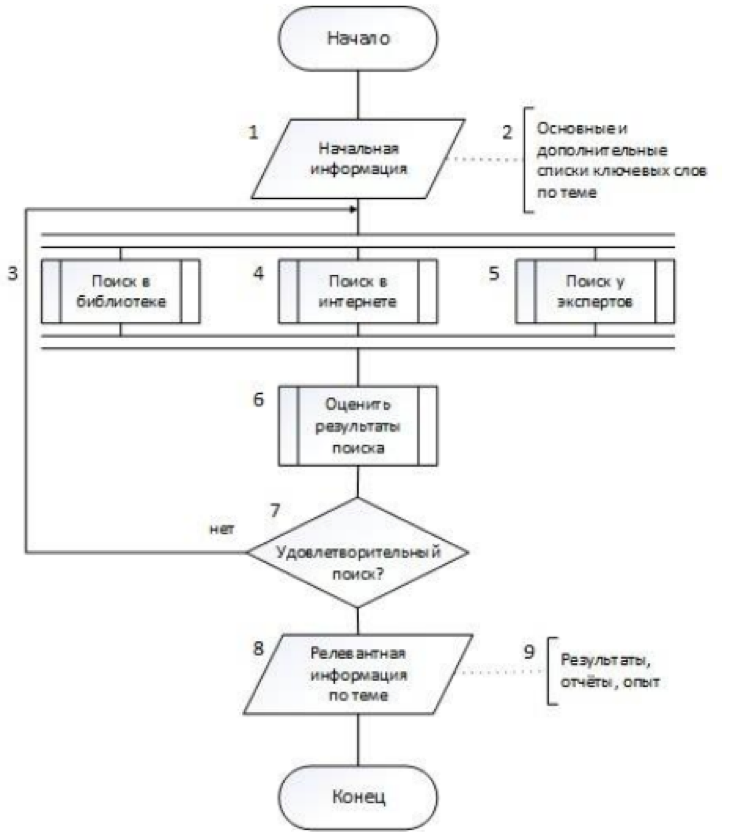
\includegraphics[width=0.7\textwidth]{images/searchinfo/1.png}
      \caption{Алгоритм поиска информации}
      \label{searchinfo:1}
    \end{figure}

    \pagebreak

	На рисунке \ref{searchinfo:2} представлен алгоритм поиска информации в библиотеке
(декомпозиция блока 4).

	\begin{figure}[h!]
		\centering
		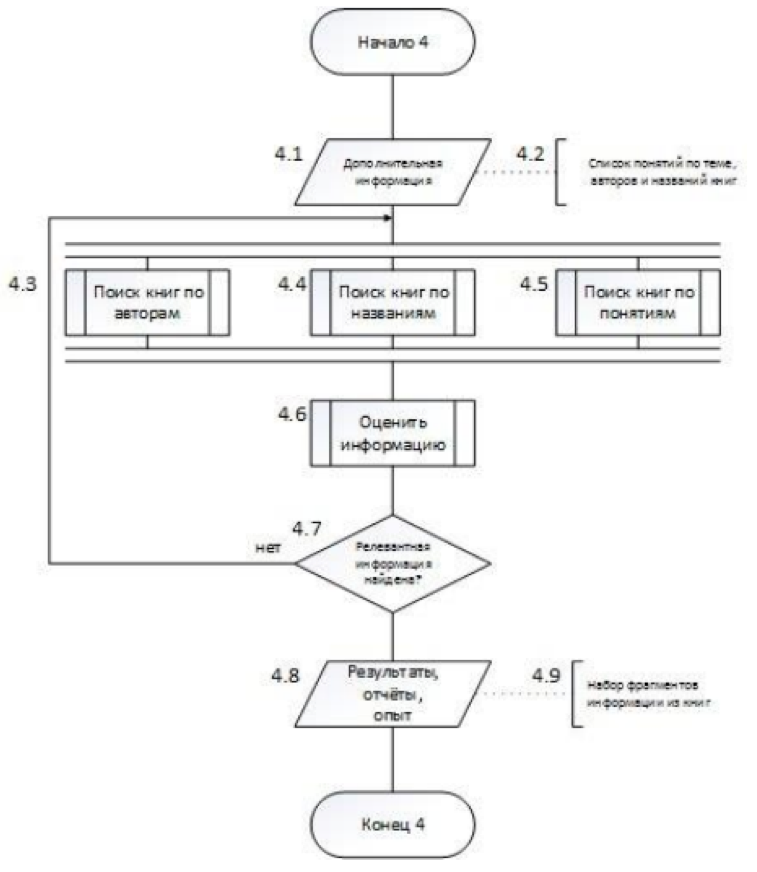
\includegraphics[width=0.7\textwidth]{images/searchinfo/2.png}
		\caption{Алгоритм поиска информации в библиотеке}
		\label{searchinfo:2}
    \end{figure}

    \pagebreak

	На рисунке \ref{searchinfo:3} представлен алгоритм поиска информации в Интернете
(декомпозиция блока 5).

	\begin{figure}[h!]
		\centering
		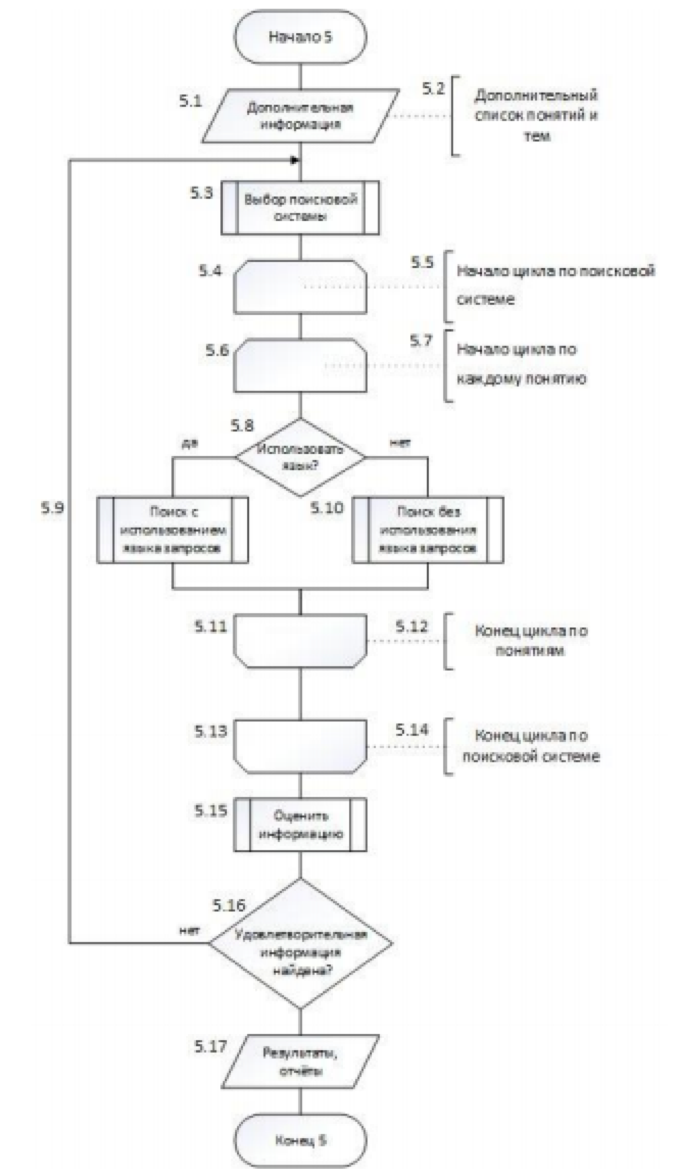
\includegraphics[width=0.7\textwidth]{images/searchinfo/3.png}
		\caption{Алгоритм поиска информации в Интернете}
		\label{searchinfo:3}
    \end{figure}

    \pagebreak

	На рисунке \ref{searchinfo:4} представлен алгоритм поиска информации у экспертов (декомпозиция блока 6).

	\begin{figure}[h!]
		\centering
		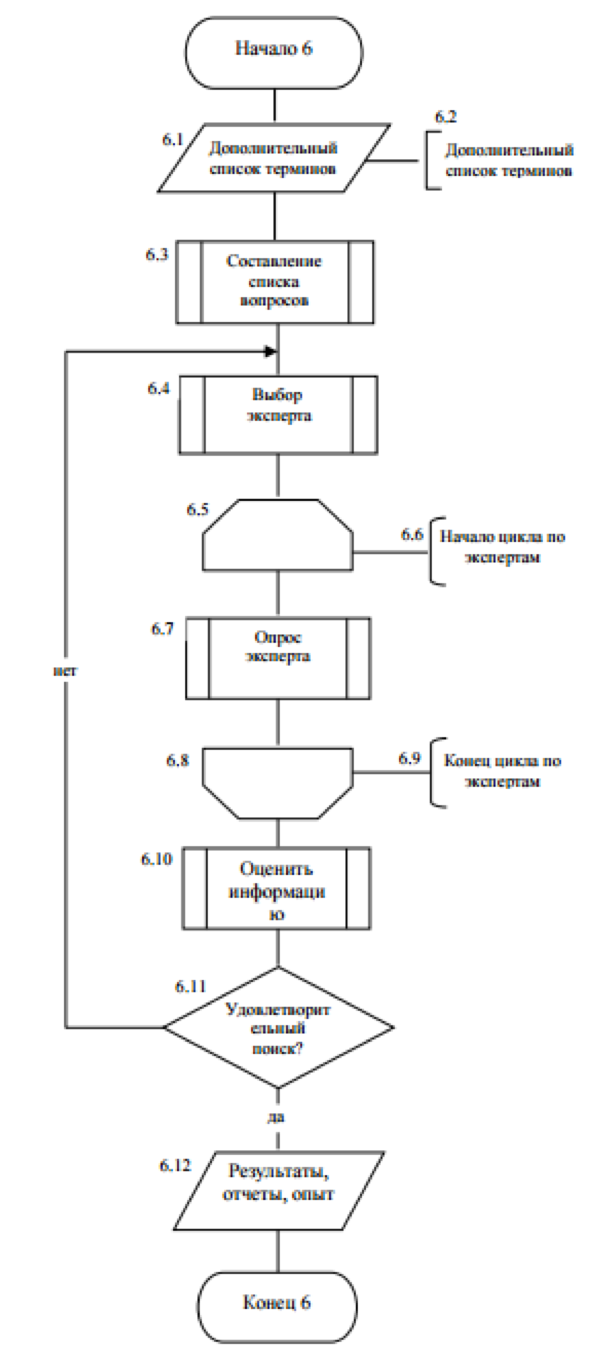
\includegraphics[width=0.5\textwidth]{images/searchinfo/4.png}
		\caption{Алгоритм поиска информации у экспертов}
		\label{searchinfo:4}
    \end{figure}

    \pagebreak

\section{Литературно-аналитический обзор}

\par

	На сегодняшний день активно разрабатываются и поддерживаются веб-сервисы, использующие для своей работы данные геоинформационных систем. Одна из разновидностей таких сервисов --- \textbf{системы анализа тепловых утечек (САТУ)}, предоставляющие информацию об уровне энергетической эффективности зданий.

	САТУ позволяют пользователям узнать оценки теплоэнергетической эффективности выбранных зданий; в некоторых случаях также возможно увидеть локализацию утечки тепла. Оценка эффективности основывается на результатах анализа тепловизионных изображений, сделанных наземно или с использованием воздушной съемки.
	
	Большинство САТУ работают со снимками крыш зданий. Это можно объяснить следующими причинами:
	\begin{itemize}
		\item простота и доступность процесса воздушной съёмки, возможность автоматизации за счёт использования БПЛА;
		\item масштабируемость системы за счет универсальности алгоритмов анализа зданий;
		\item большой охват обследуемой территории за относительно короткое время съёмки;
		\item достаточный уровень достоверности результатов для невысоких зданий, для которых рассеивание тепла незначительно.
	\end{itemize}

	Такой подход позволяет получить оценку уровня теплоэффективности для каждого здания в исследуемом районе без значительного вмешательства человека в этот процесс. При обследовании изображений автоматически учитывается различная вспомогательная информация с целью повышения точности оценки. Так, в системе HEAT, использующей ИК-изображения, данные со спутников об излучении тепла и технологию {TURN} (нормализация по температуре дорожной поверхности), конечная оценка включает в себя не только результат анализа распределения температуры, но и внешние условия, такие как температура почвы, элемент нагрева поверхности крыш в зависимости от материала и пр. Автоматизированность, кроме того, обеспечивается алгоритмами обнаружения жилых объектов на фотографиях, последующей сегментацией изображения и идентификацией этих объектов \cite{problem:heat}.

	Тем не менее, более качественный и информативный анализ требует тщательного подхода к съёмке анализируемого объекта. Съёмка фасадов зданий может дать больше полезной информации, чем съёмка крыш с воздуха. Так, при частном исследовании зданий бригады экспертов используют специальное ИК-оборудование для захвата всех деталей фасадов, поскольку в этом случае важно выявление причин утечек, что не всегда возможно сделать при помощи только снимков крыш. Существующие способы \cite{problem:detection-windows-doors}, \cite{problem:aerial-oblique}, \cite{problem:thermal-leakages-facades}, позволяющие с определённой долей вероятности выделить, а в некоторых случаях даже сформулировать \cite{problem:knowledge-based-system} причины утечек, работают именно со снимками фасадов зданий. В целом, для оценки тепловой энергоэффективности невысоких зданий достаточно изображений поверхности кровли, однако при работе с более высокими зданиями, в том числе с многоэтажными, таких снимков не будет достаточно для объективного результата. 

	В этом случае возникает вопрос о том, как автоматизировать процесс съёмки фасадов зданий. Беспилотная съёмка позволяет быстро получать данные при съёмке крыш, но в применении к фасадам зданий в городской местности такой метод реализовать практически невозможно по ряду причин (технические и юридические причины). Проявляющаяся в настоящее время в геоинформационных системах тенденция к использованию {VGI} - добровольно предоставляемой географической информации - способна решить эту проблему \cite{problem:citizens-as-sensors}. Под термином {VGI} подразумеваются принципы сбора, обработки и распространения геоданных, предоставляемых лично владельцами (пользователями, имеющими к ним доступ) \cite{problem:vgi}. Такая практика используется в проектах {OpenStreetMap}, {Google Earth}, {WikiMapia}, {Panoramio} и др. С развитием доступности Интернет по всему миру этот подход получения данных становится неоспоримо эффективным. В этой связи он может обеспечить САТУ более актуальными сведениями, а также значительно увеличить количество анализируемых объектов. 

	Для сбора и отправки {VGI}-данных можно использовать любое устройство, обладающее необходимыми датчиками и имеющее выход в Интернет.  Такой подход используется, например, в системах регистрации сейсмической активности, работающих с данными акселерометров пользовательских устройств. Для этой цели хорошо подходят смартфоны, так как они мобильны и их использование широко распространено.

	\textbf{Смартфон} --- сложное многофункциональное устройство, как правило, снабженное встроенной фото- и видеокамерой, модулем {Wi-Fi}, датчиками положения в пространстве, ускорения. Существуют портативные камеры инфракрасной съемки, представляющие из себя модули, подключаемые к смартфону. Используя эти устройства, можно сделать распределенную систему сбора информации, добровольно предоставляемой пользователями смартфонов. 


\section{Аналоги системы и их оценка}

\subsection{MyHEAT}

\par
	\textbf{MyHEAT} - система, разработанная исследовательским университетом Калгари, Канада. Система представлена веб-интерфейсом, позволяющим просмотреть тепловую карту местности, полученную в результате анализа тепловизионных аэроснимков зданий, исходные изображения зданий, а также узнать оценки их теплоэнергетической эффективности по шкале от 1 до 10 баллов, где 1 балл соответствует низкой эффективности, а 10 - высокой \cite{problem:myheat-utilities}. Для визуального представления используется картографический сервис {Google Maps} с наложением слоев с информацией об утечках тепла. При построении карты используются проприетарные алгоритмы, исключающие микроклиматическую изменчивость и геопространственные эффекты, а также учитывающие материал крыш и количество растительности на них, что повышает точность построения карт. Интерфейс системы представлен на рисунке \ref{screens:myheat}.

	\begin{figure}[h!]
      \centering
      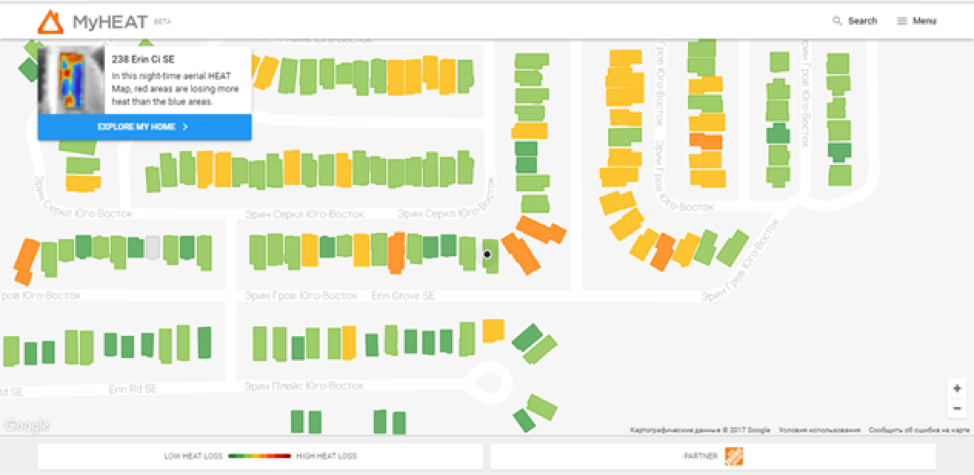
\includegraphics[width=0.9\textwidth]{images/screens/0_myheat.png}
      \caption{Внешний вид интерфейса системы MyHEAT}
      \label{screens:myheat}
    \end{figure}

\subsection{National Heat Map}

\par
	\textbf{National Heat Map} - разработка Центра по устойчивой энергетике (CSE) в Великобритании. Этот проект существует с 2010 года, данные в нём постоянно обновляются \cite{problem:nhm}. NHM позволяет получать данные по адресам зданий, в открытом доступе предоставляет интерактивную тепловую карту с выбором различных слоёв по категориям зданий (производственные, коммерческие и жилые). Эти слои представляют собой цветные изображения областей по уровням тепловыделения.

 	Данные о распределении тепла в конкретных зданиях предоставляются административным органам, а также организациям, имеющим специальную лицензию. Отличительная особенность данной системы - проработанный веб-интерфейс, который позволяет рассматривать карту по разным слоям одновременно, выделять интересующие области. Имеется возможность вывода результатов статистических расчётов по выбранной области в различных форматах (табличные, такие как {CSV}, диаграммы и графики). Такое решение подходит для случаев, когда нужен охват территории в масштабе целого континента. Однако оно не позволяет увидеть оценки для конкретных зданий в открытом виде, предоставляя лишь усреднённые показатели для комплексов зданий или отдельных улиц, районов и т. п.

 	\begin{figure}[h!]
      \centering
      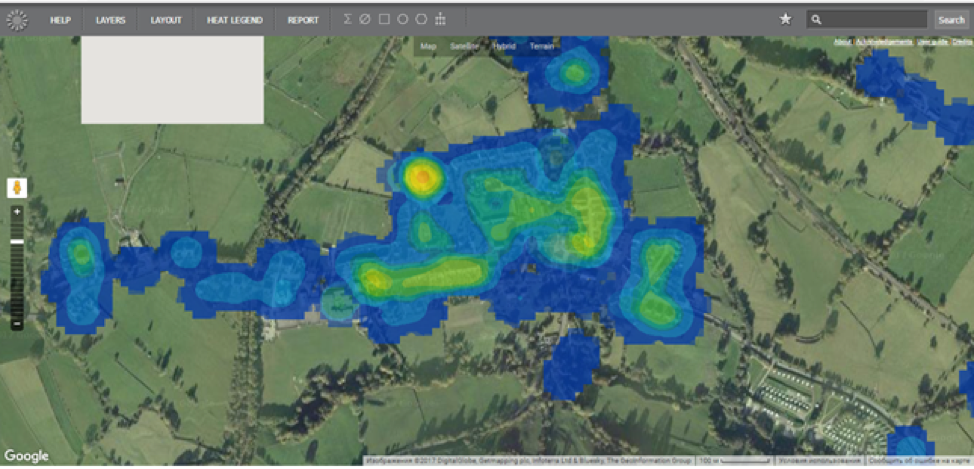
\includegraphics[width=0.9\textwidth]{images/screens/1_nhm.png}
      \caption{Внешний вид интерфейса системы National Heat Map}
      \label{screens:nhm}
    \end{figure}

\subsection{HEAT}

\par
	\textbf{HEAT} - веб-ориентированная система анализа потерь тепла, использующая тепловые аэроснимки \cite{problem:heat}. Используются стандарты {OGC} (Open Geospatial Consortium) для геопространственных сервисов, картографический сервис {Google Maps} с возможностью выбора слоя тепловых утечек. Слой представляет из себя совокупность зданий, каждое из которых окрашено в соответствии с присвоенным ему одним из десяти классов энергетической эффективности, основанных на средней температуре крыш всех зданий. Система предоставляет такую информацию, как:

	\begin{itemize}
		\item минимальная и средняя температуры поверхности крыши выбранного здания;
		\item три наиболее горячие точки на поверхности крыши;
		\item суточную стоимость отопления дома и количество выделяющегося при этом углекислого газа в зависимости от вида топлива (газ/уголь/возобновляемые источники энергии);
		\item количество топлива, его стоимость и величина выделяемого углекислого газа, которые можно сократить при условии уменьшения температуры крыши до минимальной.
	\end{itemize}

	Важной особенностью сервиса является использование решений Geographic Object Based Image Analysis ({GEOBIA}), позволяющих в автоматическом или полуавтоматическом режиме генерировать готовые к внедрению в ГИС полигоны домов, анализируя непосредственно тепловые аэроснимки, а не используя имеющиеся городские кадастровые данные. Это играет существенную роль, когда кадастровые данные недоступны, и позволяет получить доступ к информации через веб-страницу в течение недели после сбора данных.

	\begin{figure}[h!]
      \centering
      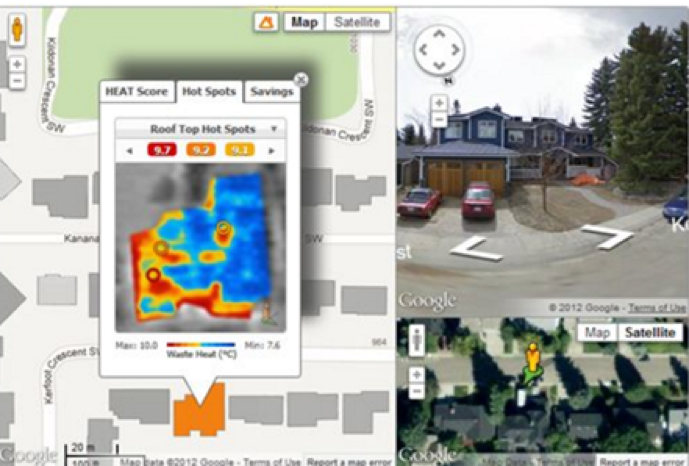
\includegraphics[width=0.9\textwidth]{images/screens/2_heat.png}
      \caption{Внешний вид интерфейса системы HEAT}
      \label{screens:heat}
    \end{figure}

\subsection{blomURBEX}

\par
	\textbf{blomURBEX} - разработка норвежской компании Blom. Представляет из себя веб-сервис, предоставляющий доступ к карте, на которую добавлены слой информации об утечках тепла и оценка, присваиваемая теплоэнергетической эффективности здания. Можно производить поиск по адресу, также предусмотрена навигация по карте. Есть возможность нанесения на карту дополнительных графической объектов и текста, сохранения результатов в файл.

\subsection{Jersey Heat Loss Map}

\par
	Интерактивная карта, разработанная службой энергоэффективности (EES) острова Джерси, ориентирована не только на городские коммунальные службы, но и на самих владельцев домов, позволяя им увидеть оценку результатов тепловизионного анализа по установленной шкале уровней тепловых утечек. Сами здания на карте представлены прямоугольниками разных цветов, соответствующих уровням этой шкалы. По каждому объекту можно получить такую информацию, как тип здания, индекс тепловых потерь и его текстовое описание. Из недостатков данной системой существенными являются отсутствие возможности увидеть изображения распределения тепла и получить статистику в произвольном масштабе.

\subsection{Оценка аналогов}

\par

	Для сравнения аналогов были выбраны критерии, по которым будет производиться оценка. Кортежная модель оценки аналогов имеет вид:

	\begin{center}
		ОА=<О(УФ), О(РТ), О(РЭ), О(ГП), О(КС), О(СР), О(ПЗ); R>, 
	\end{center} 

	где ОА --- оценка аналога, О(УФ) --- оценка учета факторов, О(РТ) --- оценка предоставления информации о распределении температур, О(РЭ) --- оценка расчёта энергии, О(ГП) --- оценка генерации полигонов, О(КС) --- оценка количества слоёв, О(СР) --- оценка выдачи статистических расчётов, О(ПЗ) --- оценка поиска зданий, R - матрица связи.

	\textbf{Учёт факторов}. Первый критерий -- учёт факторов -- подразумевает “выравнивание” результатов с учётом изменения микроклимата от одного здания к другому, учёт материалов крыш, использование алгоритмов повышения достоверности информации. Данный критерий оценивается следующим образом:
	%\noindent
	% \begin{center}
		\begin{equation*}
			I_\textup{УФ} = 
	 		\begin{cases}
	   			1, &\text{если учитывается микроклимат и материал крыши;}\\
	   			0.5, &\text{если используются статистические данные;} \\
	   			0, &\text{если дополнительные факторы не учитываются.}
	 		\end{cases}
		\end{equation*}
	% \end{center}

	\textbf{Распределение температур}. Критерий оценивается в зависимости от того, предоставляет ли выбранный аналог информацию о распределении температур по поверхности крыш зданий или нет:
	% \begin{center}
		\begin{equation*}
			I_\textup{РТ} = 
	 		\begin{cases}
	   			1, &\text{если система предоставляет информацию о распределении;} \\
	   				& \text{температуры по обследуемой поверхности здания;}\\
	   			0, &\text{если система не предоставляет такую информацию.}
	 		\end{cases}
		\end{equation*}
	% \end{center}

	\textbf{Расчет энергии}. Критерий оценивается в зависимости от предоставления системой информации о количестве энергии, затрачиваемой на отопление дома:
	% \begin{center}
		\begin{equation*}
			I_\textup{РЭ} = 
	 		\begin{cases}
	   			1, &\text{если система предоставляет информацию о количестве энергии,} \\
	   				& \text{затрачиваемой на отопление дома;}\\
	   			0, &\text{если система не предоставляет такую информацию.}
	 		\end{cases}
		\end{equation*}
	% \end{center}

	\textbf{Генерация полигонов}. Оценка производится на основе возможности системы создавать полигоны зданий, используя распознавание объектов и не прибегая к кадастровой информации.
	% \begin{center}
		\begin{equation*}
			I_\textup{ГП} = 
	 		\begin{cases}
	   			1, &\text{если система генерирует полигоны;}\\
	   			0, &\text{если система не генерирует полигоны.}
	 		\end{cases}
		\end{equation*}
	% \end{center}

	\textbf{Количество доступных слоев}. При отображении карты на нее могут накладываться слои с различной вспомогательной информацией, статистическими данными и выбранными фильтрами. Оценка этого критерия производится следующим образом:
	% \begin{center}
		\begin{equation*}
			I_\textup{КС} = 
	 		\begin{cases}
	   			1, &\text{если имеется три и более слоёв;}\\
	   			0.5, &\text{если имеется два слоя;} \\
	   			0, &\text{если имеется один слой.}
	 		\end{cases}
		\end{equation*}
	% \end{center}

	\pagebreak

	\textbf{Статистические расчеты}. Оценка этого критерия производится в зависимости от возможности предоставления системой статистических расчетов:
	% \begin{center}
		\begin{equation*}
			I_\textup{СР} = 
	 		\begin{cases}
	   			1, &\text{если система предоставляет статистические расчёты по выбранной;} \\
	   			 & \text{территории с учётом параметров, характеризующих здания} \\
	   			 & \text{и специфику местности;}\\
	   			0, &\text{если система не предоставляет такую информацию.}
	 		\end{cases}
		\end{equation*}
	% \end{center}

	\textbf{Поиск зданий}. Оценка критерия производится следующим образом:
	% \begin{center}
		\begin{equation*}
			I_\textup{СР} = 
	 		\begin{cases}
	   			1, &\text{если предусмотрена возможность поиска зданий по адресу;}\\
	   			0, &\text{если такая возможность не предусмотрена.}
	 		\end{cases}
		\end{equation*}
	% \end{center}

	Оценка аналогов будет производиться по следующей формуле:
	\begin{center}
		ОА = О(УФ)$\cdot\alpha$(УФ)+О(РТ)$\cdot\alpha$(РТ)+О(РЭ)$\cdot\alpha$(РЭ)+

		+О(ГП)$\cdot\alpha$(ГП)+О(КС)$\cdot\alpha$(КС)+О(СР)$\cdot\alpha$(СР)+О(ПЗ)$\cdot\alpha$(ПЗ),
	\end{center}
	где $\sum\limits_{i=1}^{n}{\alpha_{i}} = 1$, $\alpha_{i}$ --- весовой коэффициент $i$-го критерия. \\

\par

	\textbf{Определение весовых коэффициентов критериев}.

	При методе попарных сравнений используется шкала словесных определений уровня важности, где каждому определению ставится в соответствие число (таблица \ref{table:scale})

	\begin{table}[h!]
		\begin{raggedright}
			\caption{Шкала уровней важности}
			\begin{tabular}{ | p{0.7\textwidth} | p{0.2\textwidth} | }
				\hline
				Уровень важности & Количественное значение \\
				\hline
				Равная важность & 1 \\
				\hline
				Промежуточное значение между равенством и слабым превосходством & 2 \\
				\hline
				Умеренное превосходство & 3 \\
				\hline
				Промежуточное значение между слабым и сильным превосходством & 4 \\
				\hline
				Существенное или сильное превосходство & 5 \\
				\hline
				Промежуточное значение между сильным и значительным превосходством & 6 \\
				\hline
				Значительное (большое) превосходство & 7 \\
				\hline
				Промежуточное значение между значительным и абсолютным превосходством & 8 \\
				\hline
				Абсолютное превосходство & 9 \\
				\hline
			\end{tabular}
			\label{table:scale}
		\end{raggedright}
	\end{table}

	\pagebreak

	Оценка аналогов производилась с использованием методики Томаса Саати. В таблице \ref{table:est} представлена матрица попарного сравнения критериев.

	\begin{table}
		\begin{raggedright}
			\caption{Оценка весовых коэффициентов критериев}
			\begin{tabular}{ | p{0.3\textwidth} | l | l | l | l | l | l | l | c | c | }	
				\hline
				   & УФ & РТ & РЭ & ГП & КС & СР & ПЗ & $\Sigma$ & $\alpha$ \\
				\hline
				УФ &1   &2   &3   &4   &5   &6   &8   &29.00 &0.26 \\
				\hline
				РТ &1/2 &1   &2   &4   &6   &7   &9   &29.50 &0.26 \\
				\hline
				РЭ &1/3 &1/2 &1   &3   &5   &5   &7   &21.83 &0.19 \\
				\hline
				ГП &1/4 &1/4 &1/3 &1 &  3   &3   &6   &13.83 &0.12 \\
				\hline
				КС &1/5 &1/6 &1/5 &1/3 &1   &2   &5   &8.90  &0.08 \\
				\hline
				СР &1/6 &1/7 &1/5 &1/3 &1/2 &1   &4   &6.34  &0.06 \\
				\hline
				ПЗ &1/8 &1/9 &1/7 &1/6 &1/5 &1/4 &1   &2.00  &0.02 \\
				\hline
				ЭР &1/9 &1/9 &1/8 &1/7 &1/6 &1/6 &1/2 &1.32  &0.01 \\
				\hline 
				\multicolumn{8}{|c|}{$\Sigma\Sigma$}           &112.73 &1   \\
				\hline
			\end{tabular}
			\label{table:est}
		\end{raggedright}
	\end{table}

	В таблице \ref{table:critval} приведены оценки аналогов по выбранным критериям.

	\begin{table}[h!]
		\begin{raggedright}
			\caption{Показатели критериев аналогов}
			\begin{tabular}{ | p{0.43\textwidth} | l | l | l | l | l | l | l | l | }	
				\hline
				  	                        &УФ  &РТ &РЭ &ГП &КС  &СР &ПЗ &ЭР \\
				\hline
					Jersey Heat Loss Map 	&0   &0  &0  &0  &0   &0  &1 &0 \\
				\hline
					HEAT 					&1   &1  &1  &1  &0,5 &0  &0 &0 \\
				\hline
					MyHEAT 					&1   &1  &1  &1  &0   &0  &1 &0 \\
				\hline
					BlomURBEX 				&0   &0  &0  &0  &0,5 &0  &1 &1 \\
				\hline
					National Heat Map 		&0.5 &0  &1  &0  &1   &1  &1 &1 \\
				\hline
			\end{tabular}
			\label{table:critval}
		\end{raggedright}
	\end{table}

	Взвешенные оценки аналогов представлены в таблице \ref{table:weightedest}.

	\begin{table}[h!]
		\begin{raggedright}
			\caption{Оценки аналогов по критериям}
			\begin{tabular}{ | l | l | l | l | l | l | l | l | l | l | }	
				\hline
				 	&УФ &РТ &РЭ &ГП &КС &СР &ПЗ &ЭР &$\alpha$\\
				\hline
					&0.26 &0.26 &0.19 &0.12 &0.08 &0.06 &0.02 &0.01 &1.00 \\
				\hline
					Jersey Heat Loss Map &0 &0 &0 &0 &0 &0 &0.02 &0 &0.02 \\
				\hline
					HEAT &0.26 &0.26 &0.19 &0.12 &0,04 &0 &0 &0 &0.87 \\
				\hline
					MyHEAT &0.26 &0.26 &0.19 &0.12 &0 &0 &0.02 &0 &0.85 \\
				\hline
					BlomURBEX &0 &0 &0 &0 &0,04 &0 &0.02 &0.01 &0.07 \\
				\hline
					National Heat Map &0.13 &0 &0.19 &0 &0.08 &0.06 &0.02 &0.01 &0.49 \\
				\hline
			\end{tabular}
			\label{table:weightedest}
		\end{raggedright}
	\end{table}

	Наиболее высокую оценку получил аналог HEAT, целесообразно рассматривать его в качестве прототипа.

\section{Критика прототипа}

\par
	В результате оценки аналогов наилучший результат получила система HEAT Университета Калгари, Канада. Основные ее преимущества - использование алгоритмов повышения достоверности результатов, автоматическая генерация полигонов зданий.
	
	Существенный недостаток системы HEAT --- отсутствие возможности работы с пользовательскими данными. Не предусмотрена функция загрузки снимков и вспомогательных данных с пользовательских устройств (в частности, со смартфонов) и их последующая обработка. Доработка этих возможностей позволит наполнить систему более полной и актуальной информацией в соответствии с принципами {VGI}. 

\section{Уточнение целей и задач}

\par

	Глобальная цель работы --- увеличить количество источников данных для обследования жилых зданий с целью оценки их тепловой энергоэффективности.

	Локальная цель --- разработать программный интерфейс ({API}), позволяющий подключать к системе приложения сторонних разработчиков на различных устройствах.

	Задачи, которые необходимо решить для достижения поставленной цели:

	\begin{itemize}
		\item выполнить аналитический обзор имеющихся в мире информационных систем, выполняющих задачу оценки тепловой энергоэффективности;
		\item провести анализ используемых в этих системах технологий, которые применяются для получения исходных данных;
		\item обнаружить среди обозреваемых систем и технологий наиболее совершенные с точки зрения поставленной в данной работе цели и выделить прототип разрабатываемой системы;
		\item разработать пакет моделей на создание улучшенной информационной системы;
		\item выполнить внешнее и внутреннее проектирование искомой системы (API САТУ);
		\item реализовать программное решение искомой системы (API САТУ).
	\end{itemize}

%\section{Аналоги по подсистеме}

%\textcolor{red}{Раздел в доработке.}

\section{Результаты и выводы по главе 1}

\par

	Проведён поиск информации об используемых решениях в области систем анализа тепловых утечек жилых зданий. Выполнен обзор литературных источников и существующих аналогов таких систем, сформулировано их общее описание. Среди аналогов на основе оценки наиболее существенных факторов выявлен прототип. На основании критики предложена доработка прототипа. Определены цели и задачи данной работы.


\chapter{Моделирование}
\label{chap:models}

\section{Концептуальная модель}

\textbf{Система анализа тепловых утечек} --- программный комплекс, выполняющий следующие основные функции:

\begin{itemize}
	\item оценка энергетической эффективности зданий городской застройки;
	\item выдача результатов оценивания по запросу;
	\item обработка ИК снимков;
	\item упрощение процесса проведения ИК съёмки пользователями.
\end{itemize}

\textbf{Пути реализации основных функций:}

\begin{itemize}
	\item обнаружение критичных областей и вычисления средних значений показателей распределения тепла по ИК снимкам;
	\item предоставление веб-доступа к результатам обследования;
	\item геометрическая коррекция изображений и учета внешних условий съёмки;
	\item программное обеспечение процесса проведения ИК съемки.
\end{itemize}
 
\textbf{Структурная основа реализации:}

\begin{itemize}
	\item методы статистического анализа;
	\item способы визуализации данных;
	\item алгоритмы нормализации ИК снимков по инвариантным признакам спутниковых снимков;
	\item клиент-серверная архитектура.
\end{itemize}

\textbf{Направленность функционирования системы}: обеспечение информационной поддержки процесса обнаружения, обследования, контроля и устранения тепловых утечек.
 
\textbf{Цель функционирования системы}: повышение качества обследования жилых объектов на предмет тепловой энергоэффективности. \\
 
\textbf{Программный интерфейс (API)} для системы анализа тепловых утечек городской застройки.

\begin{enumerate}
 
	\item \textbf{Основные функции}:

	\begin{enumerate}
		\item сбор данных; \label{cm:f:1}
		\item унификация данных, поступающих в систему анализа; \label{cm:f:2}
		\item обеспечение их корректности; \label{cm:f:3}
		\item обеспечение доступности данных для системы анализа; \label{cm:f:4}
		\item предоставление результатов анализа клиентским приложениям. \label{cm:f:5}
	\end{enumerate}

	\item \textbf{Пути реализации основных функций}:

	\begin{enumerate}
		\item приём пакетов данных от различных источников;
		\item преобразование данных в одинаковый формат;
		\item проверка пакетов входных данных на соответствие требованиям;
		\item взаимодействие с БД системы анализа;
		\item обработка внешних запросов на результаты анализа утечек.
	\end{enumerate}

	\item \textbf{Структурная основа реализации}:

	\begin{enumerate}
		\item для функций \ref{cm:f:1}, \ref{cm:f:5}: сетевые протоколы обмена информацией;
		\item для функции \ref{cm:f:2}: требования системы анализа тепловых утечек;
		\item для функции \ref{cm:f:3}: методы фильтрации нежелательного контента;
		\item для функции \ref{cm:f:4}: централизованный подход к управлению данными в СУБД.
	\end{enumerate}

	\item \textbf{Направленность функционирования системы}: расширение географической области, охватываемой системой анализа и увеличение числа пользователей системы анализа.

	\item \textbf{Цели функционирования системы}: предоставление набора функций, реализуемых системой анализа тепловых утечек, сторонним программам вне зависимости от их платформы и аппаратного обеспечения.

\end{enumerate}

\section{Системно-структурная модель}

\par 
	На рисунке \ref{ssm:0} изображена системно-структурная модель системы анализа тепловых утечек. Внедрение в неё новых структурных элементов -- программного интерфейса и мобильного приложения -- приводит к изменению состава таких подсистем, как веб-приложение и модуля работы с ИК изображениями. Модели этих подсистем представлены на рисунках [\ref{ssm:1}, \ref{ssm:3}] соответственно.

	 \begin{figure}[h!]
      \centering
      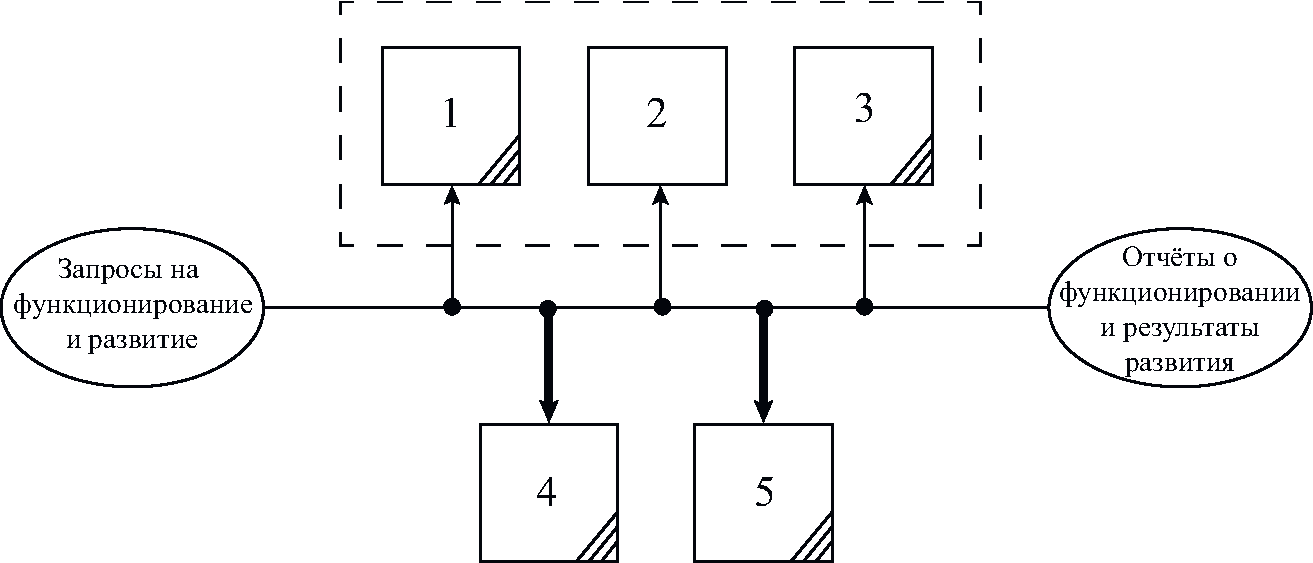
\includegraphics[width=0.9\textwidth]{images/ssm/0}
      \caption{Системно-структурная модель системы анализа тепловых утечек}
      \label{ssm:0}
    \end{figure}

\par 
	Обозначения к рисунку \ref{ssm:0}: 1 - веб-приложение, 2 - подсистема управления данными, 3 - модуль работы с ИК изображениями, 4 - мобильное приложение, 5 - программный интерфейс (API).

	Структурные компоненты web-приложения представлены разделами, с которыми работают его пользователи (рисунок \ref{ssm:1}). Работа каждого раздела обеспечивается web-сервером и множеством программных сценариев, генерирующих динамические web-страницы, содержащие информацию, соответствующую названию раздела.

\pagebreak

	\begin{figure}[t!]
      \centering
      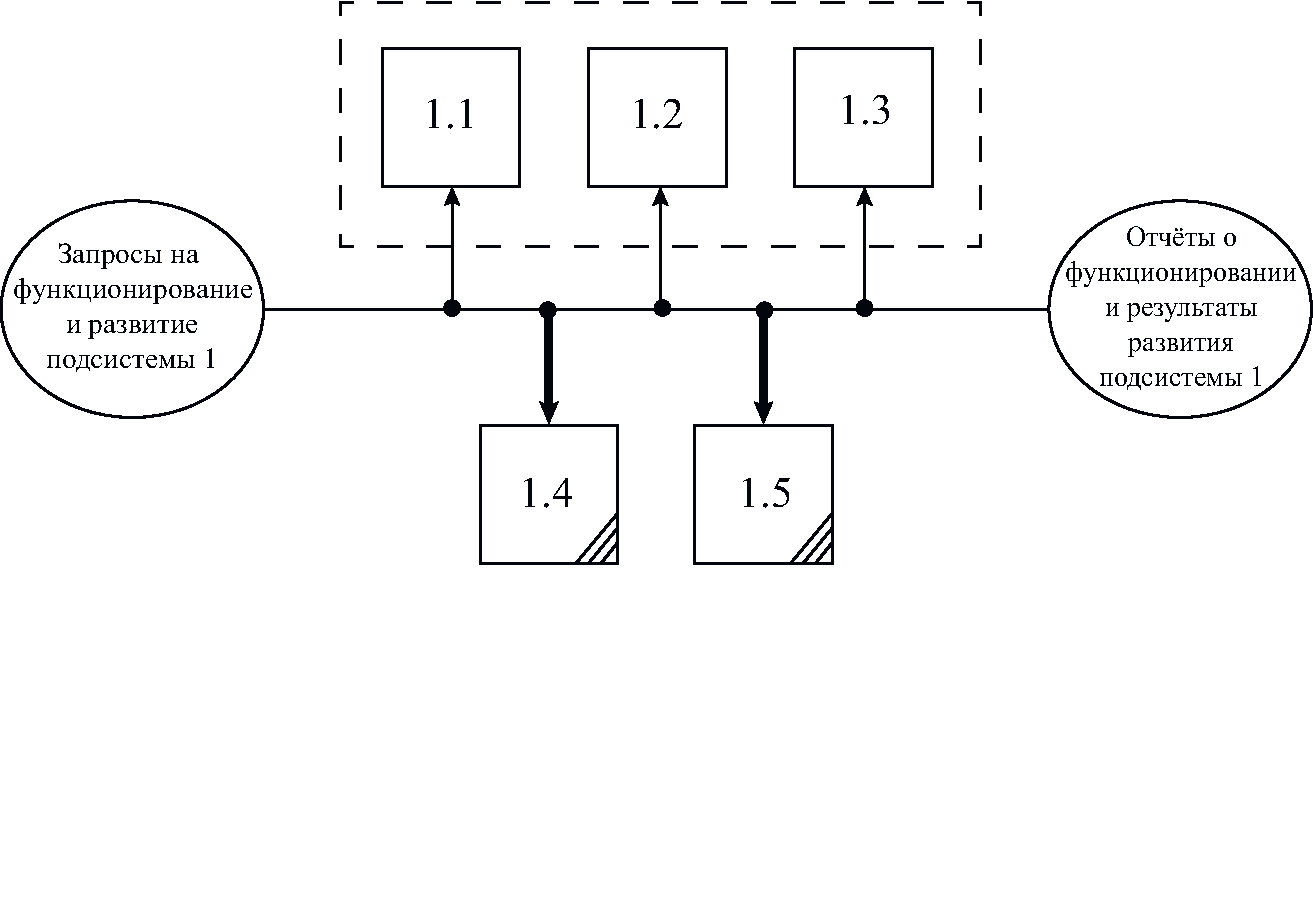
\includegraphics[width=0.9\textwidth]{images/ssm/1}
      \caption{Системно-структурная модель веб-приложения}
      \label{ssm:1}
    \end{figure}

\par
	Обозначения к рисунку \ref{ssm:1}: 1.1 - блок отображения карты, 1.2 - блок отображения оценок энергоэффективности и энергозатрат, 1.3 - блок представления изображений, 1.4 - раздел «личного кабинета», 1.5 - раздел загрузки пользовательских данных.

	Компоненты модуля работы с ИК изображениями (рисунок \ref{ssm:3}) разделены по характеру выполняемых преобразований: подсистема 3.1 решает задачу распознавания зданий с ИК аэроснимков, описанную в \cite{problem:heat}, процедуры обработки в подсистеме 3.2 устраняют отклонения, вызванные локальными изменениями климата, на снимках, подсистема 3.3 использует алгоритмы математической статистики для итоговых расчётов.

	В связи с тем, что в систему анализа тепловых утечек внедряется новый вид съёмки, очевидно, что некоторые подсистемы претерпят изменения, которые отражены в алгоритмических моделях. Подсистемы 3.1 и 3.2 являются исключениями, поскольку для наземной съёмки отдельных зданий они не актуальны. Многие задачи обработки наземных снимков берут на себя программные клиенты - мобильные приложения.

\pagebreak

	Обозначения к рисунку \ref{ssm:3}: 3.1 - подсистема фотограмметрической обработки ИК снимков, 3.2 - подсистема коррекции по микроклиматическим условиям, 3.3 - подсистема расчёта оценки энергоэффективности.

	\begin{figure}[t!]
      \centering
      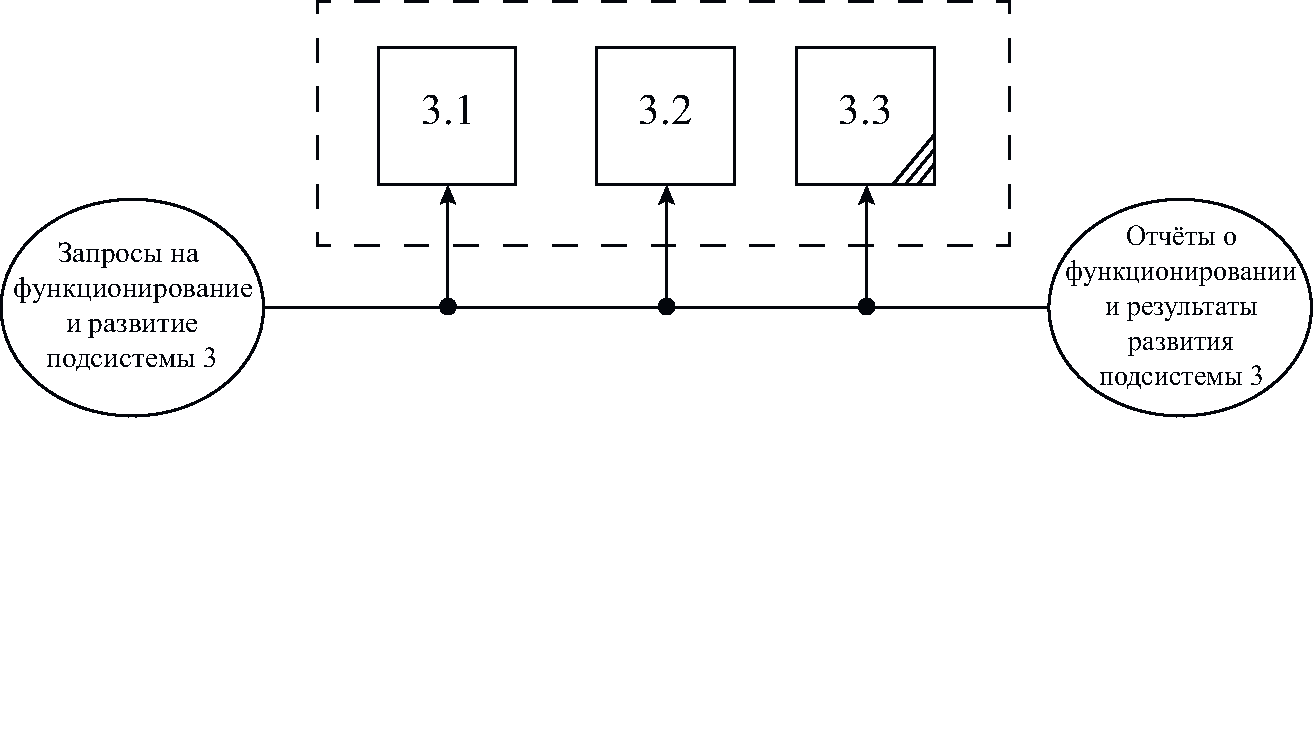
\includegraphics[width=0.9\textwidth]{images/ssm/3}
      \caption{Системно-структурная модель модуля работы с ИК изображениями}
      \label{ssm:3}
    \end{figure}

\par
	В модели программного интерфейса системы анализа тепловых утечек, представленной на рисунке \ref{ssm:5}, в качестве подсистем прототипа были взяты стандартные компоненты, участвующие в работе большинства API относительно крупных программных комплексов. 
	
	В рамках системы анализа тепловых утечек специфика API заключается в наличии подсистемы 5.5. Это связано с характерными особенностями данных, поступающих в систему. Например, в систему могут поступать данные с ИК камер различных производителей, и, кроме того, данные различных типов съёмки. Расширение спектра возможных источников данных - одна из причин внедрения API в основную систему.

\pagebreak

	\begin{figure}[t!]
      \centering
      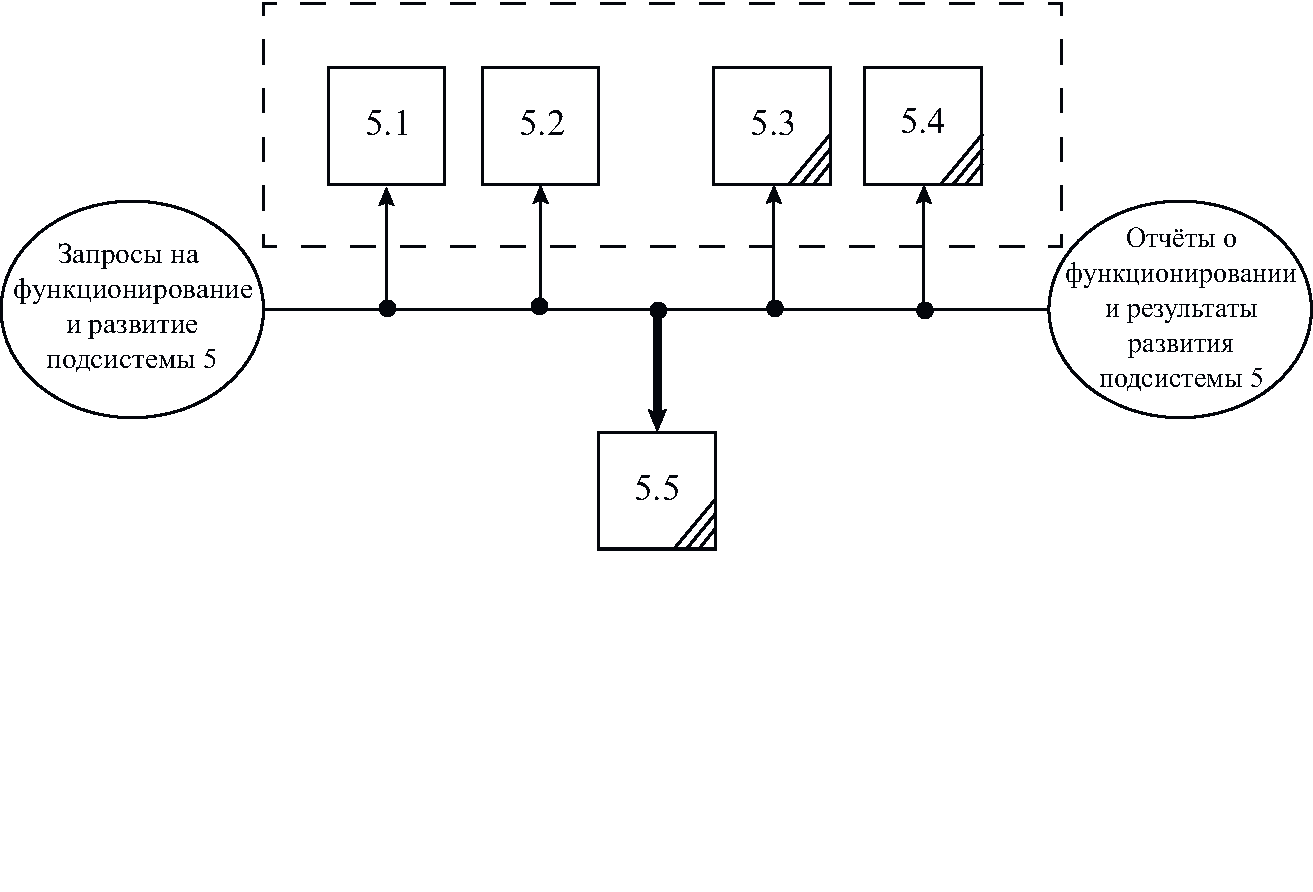
\includegraphics[width=0.9\textwidth]{images/ssm/5}
      \caption{Системно-структурная модель программного интерфейса}
      \label{ssm:5}
    \end{figure}

    Обозначения к рисунку \ref{ssm:5}: 5.1 - подсистема приёма запросов и отправки данных,  5.2 - подсистема аутентификации пользователей, 5.3 - подсистема формирования запросов к БД, 5.4 - подсистема валидации данных, 5.5 - подсистема унификации и форматирования данных.

\section{Функционально-структурная модель}

\par
	Функционально-структурная модель предлагаемого решения построена при помощи пакета {Computer Associates ERwin Process Modeler 7.3}. Модели выполнены в соответствии с методологией {IDEF0}. Диаграммы модели приведены в приложении \ref{app-fsm}.

	Все функции, выполняемые системами анализа тепловых утечек, можно объединить в один функциональный блок “Оценить энергетическую эффективность зданий”, как показано на диаграмме, изображенной на рисунке \ref{fsm:0}. Рассмотрение функциональной структуры системы в целом важно при моделировании разрабатываемого программного интерфейса, поскольку это даёт представление о взаимосвязи информационных потоков между смежными функциями всей системы, а также с её внешней средой.

\par
    Диаграмма декомпозиции 1 уровня включает в себя набор основных функций, которые выполняются подсистемами, перечисленными в системно-структурной модели \ref{fsm:1}. Так, функциональный блок \texttt{A3} выполняется программным интерфейсом (подсистема 5, рисунок \ref{ssm:5}). Некоторые подсистемы могут участвовать в работе нескольких функций. Например, за работу блоков \texttt{A2} и \texttt{A6} отвечает мобильное приложение (подсистема 3, рисунок \ref{ssm:3}).

	Описание математических алгоритмов содержится в некоторых алгоритмических моделях, приведённых в разделе \ref{sec:models:algo}. Под клиентскими приложениями понимается ПО, которое отображает карты энергоэффективности зданий (в частности, мобильное и web-приложения).

\par
    На рисунке \ref{fsm:2} представлена диаграмма декомпозиции блока \textit{“Отправить снимки на сервер”}. Все функциональные блоки в этой диаграмме задействуют API, поэтому она представляет наибольший интерес среди остальных блоков узла \texttt{A0}.

\section{Алгоритмическая модель}
\label{sec:models:algo}
	
\par
	В разделе \ref{sec:models:algo:before} приведены алгоритмы процессов работы системы до внедрения в неё новых подсистем. В разделе \ref{sec:models:algo:after} представлены алгоритмы, в которых происходят наиболее существенные изменения после внедрения внедряемых подсистем, а также алгоритм работы разрабатываемого программного интерфейса.

\pagebreak

\subsection{Алгоритмическая модель прототипа}
\label{sec:models:algo:before}

	\begin{figure}[h!]
      \centering
      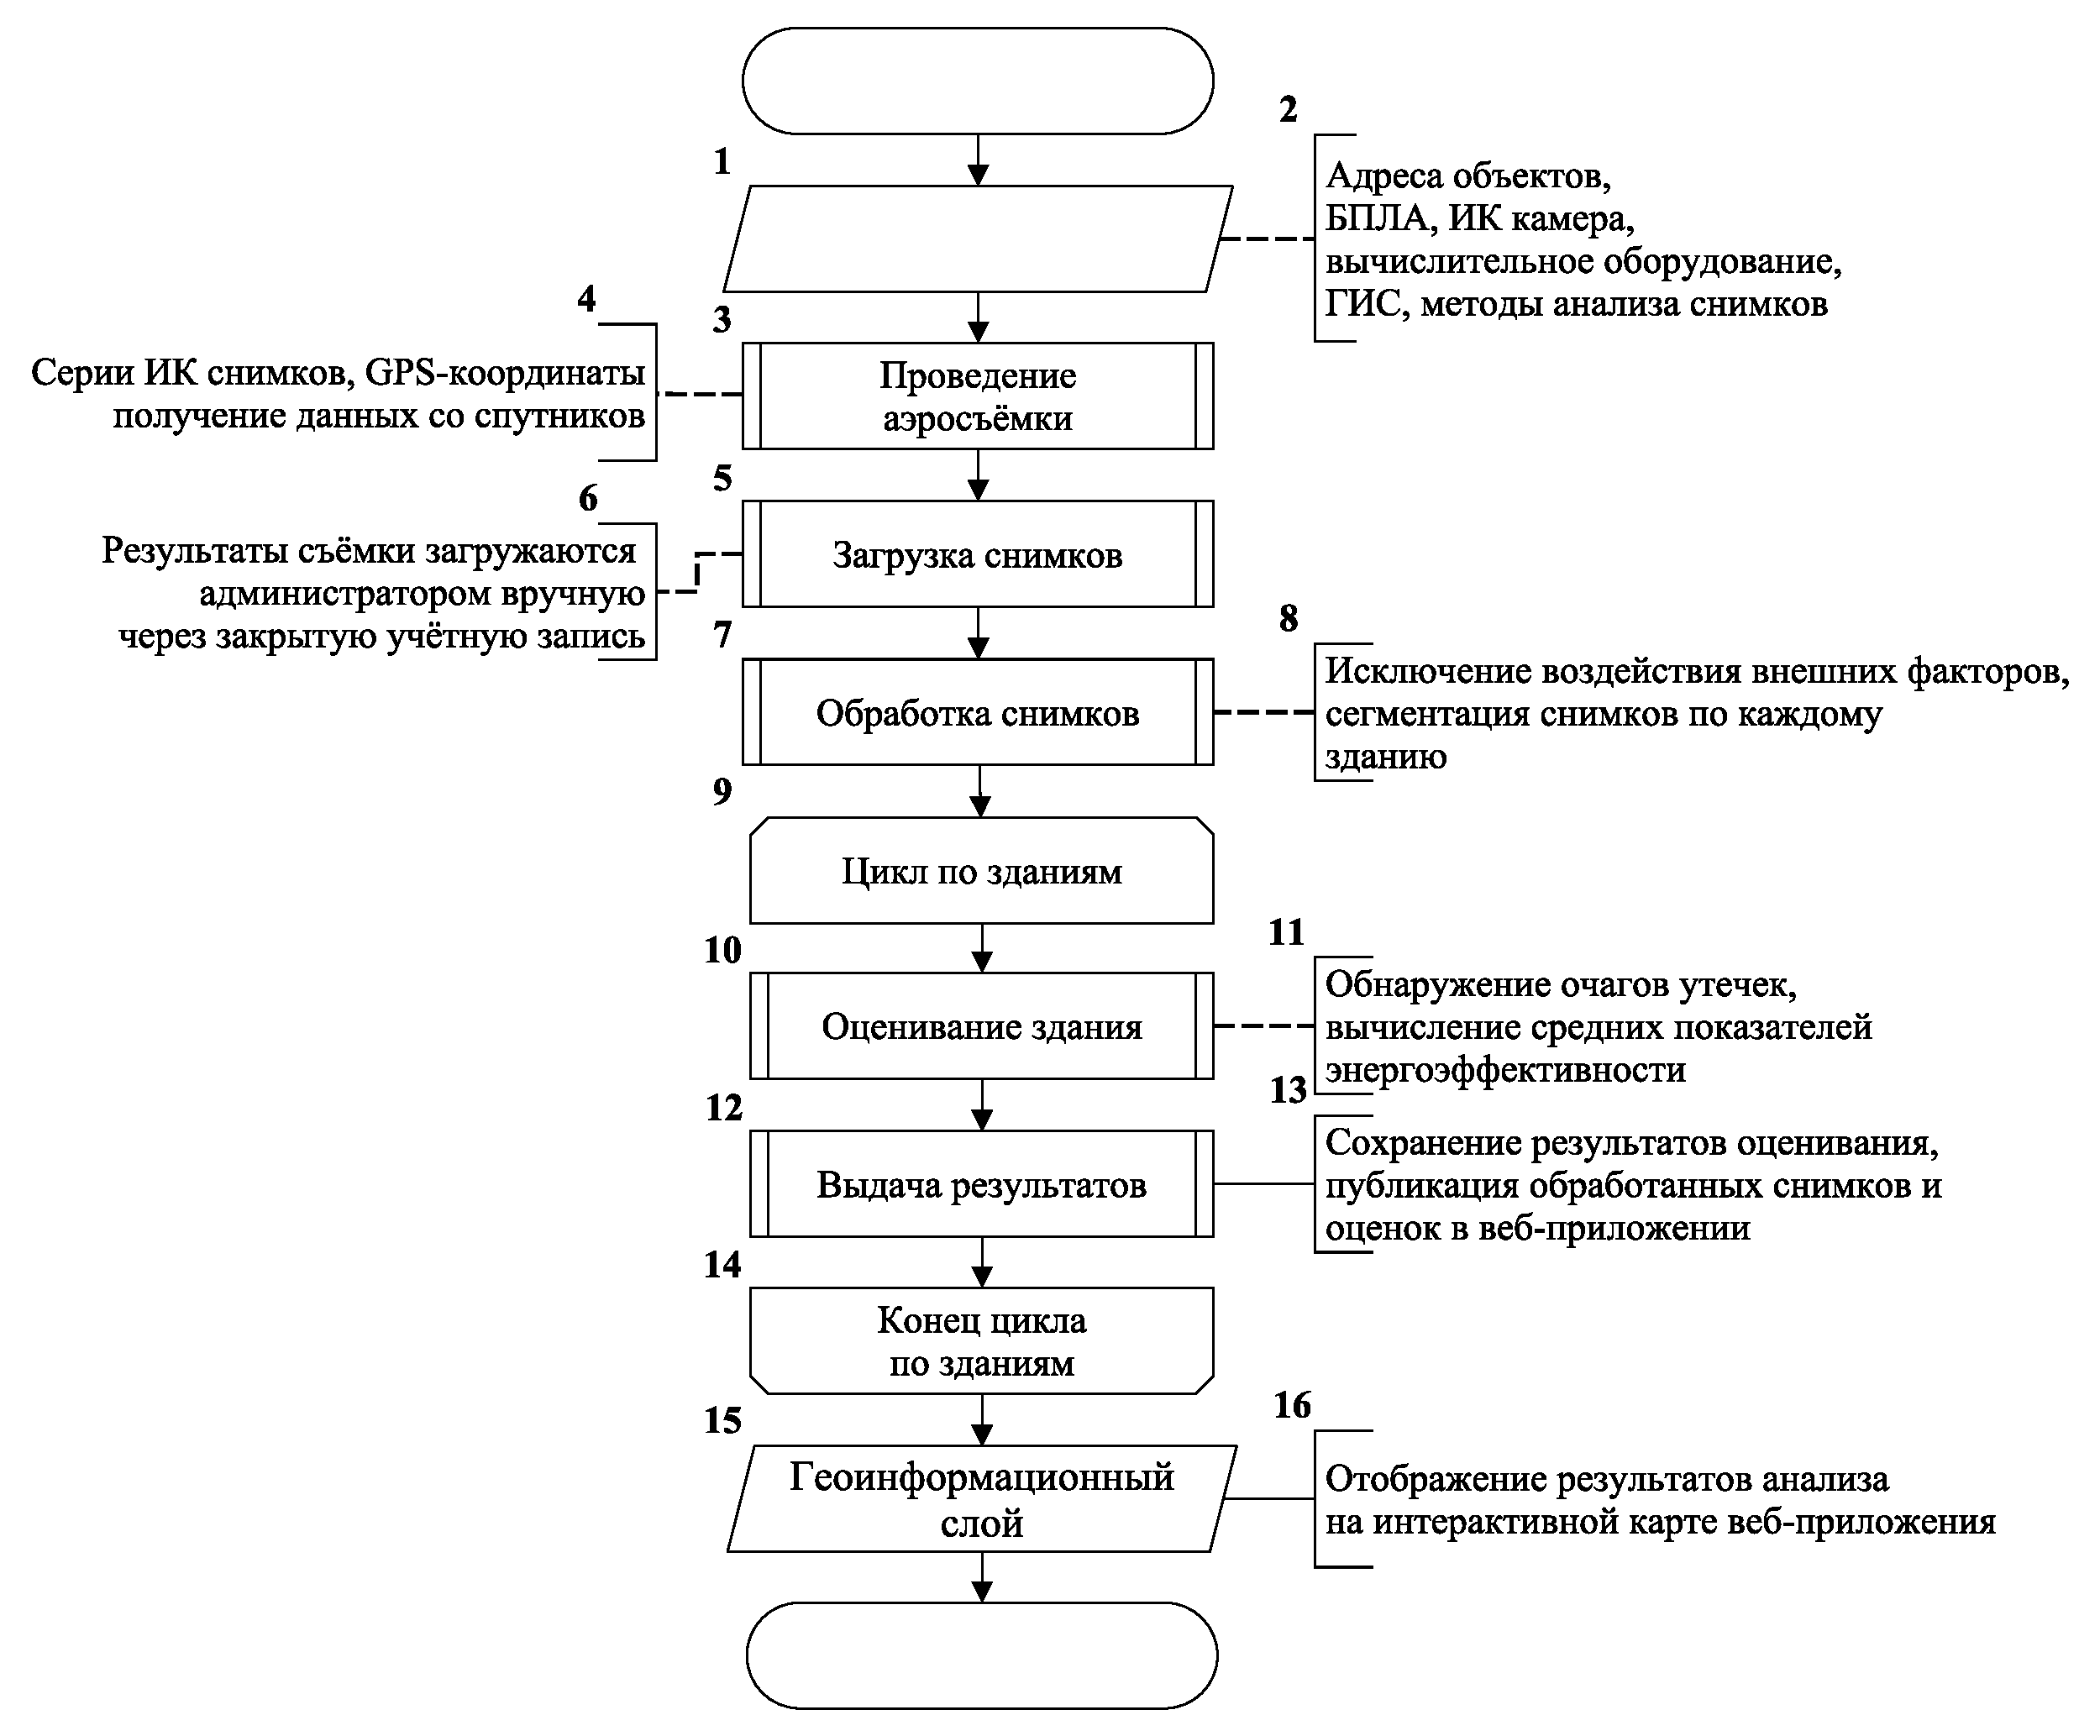
\includegraphics[width=0.9\textwidth]{images/am/am0_before}
      \caption{Алгоритм исследования утечек в жилых зданиях (для прототипа)}
      \label{am:before:common}
    \end{figure}

\pagebreak

	\begin{figure}[h!]
      \centering
      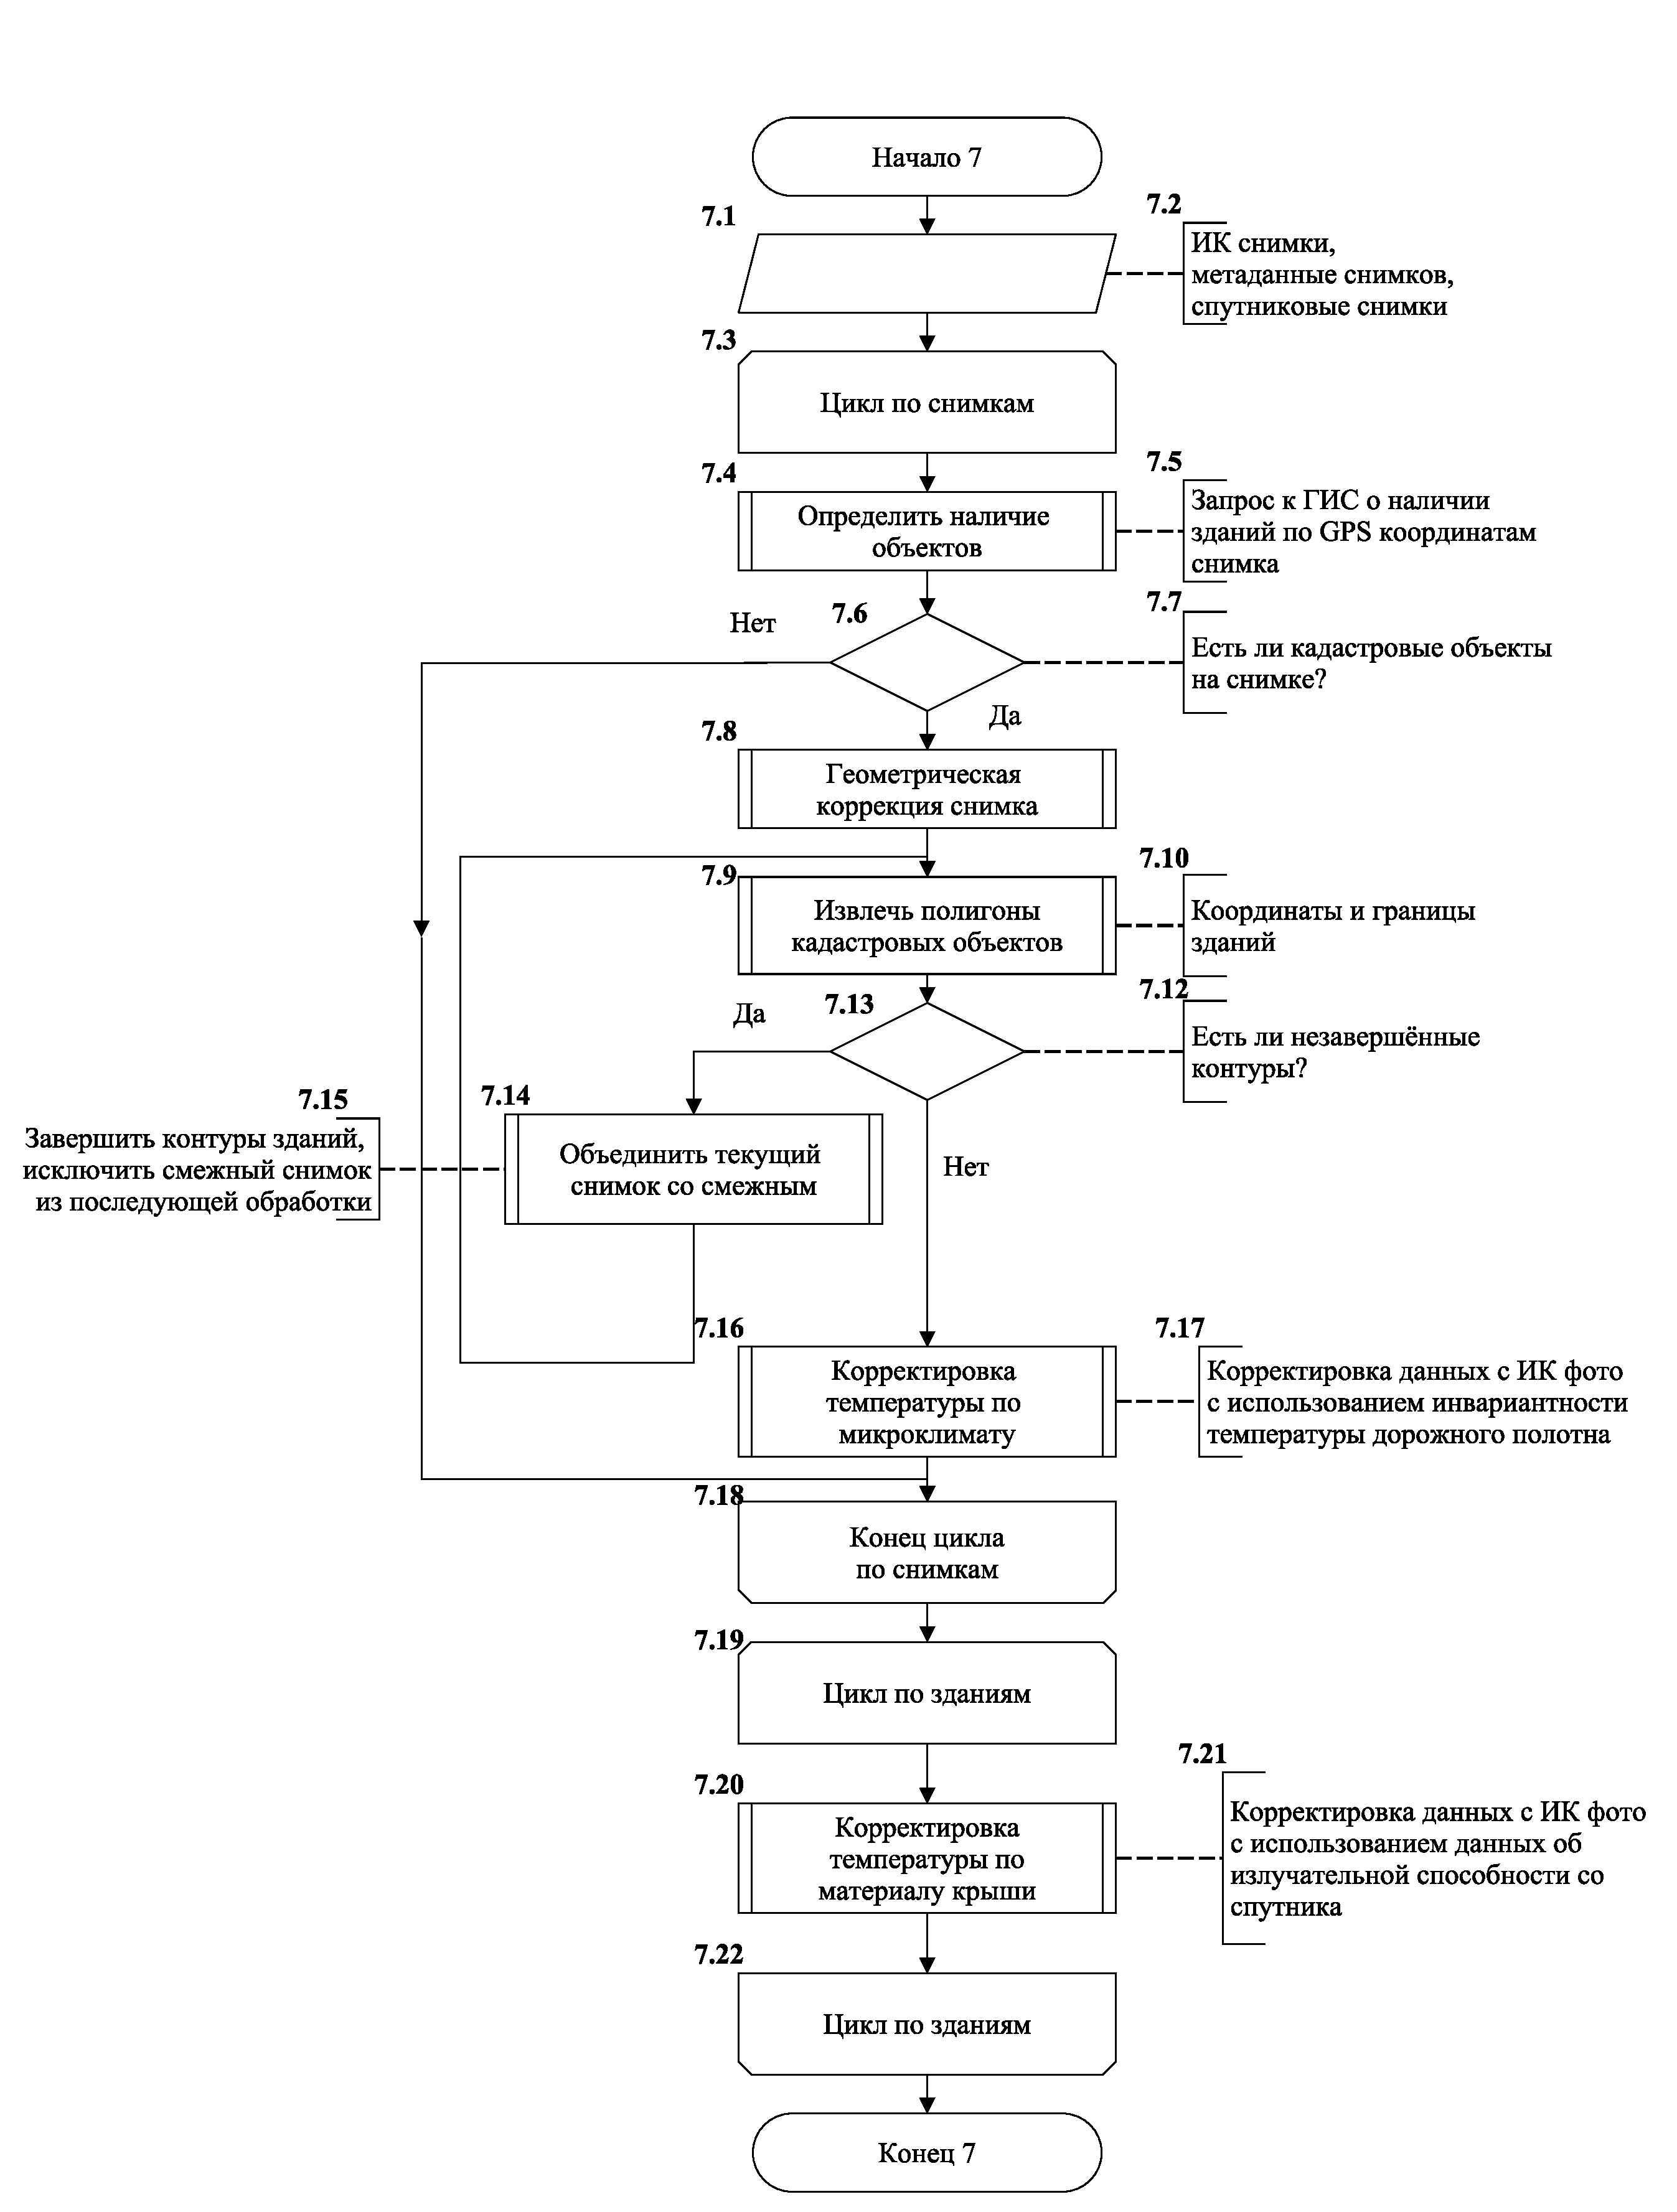
\includegraphics[width=0.9\textwidth]{images/am/am01_before}
      \caption{Алгоритм обработки аэроснимков (для прототипа)}
      \label{am:before:aero}
    \end{figure}    



\subsection{Алгоритмическая модель предлагаемого решения}
\label{sec:models:algo:after}

\par
	В связи с тем, что предлагаемая система предполагает два вида съёмки, изменяется основной алгоритм исследования утечек жилых зданий для расчёта оценки их энергоэффективности (рисунок \ref{am:after:common}). Возникает проблема, связанная с тем, что одно здание может быть отснято несколько раз, причём разным способом. Для решения этой проблемы следует проводить интегральную (итоговую) оценку, представленную в алгоритме процессом 20. Более детальное описание этого процесса описывает алгоритм, приведённый на рисунке 
	\ref{am:after:integral}.

	\begin{figure}[h!]
      \centering
      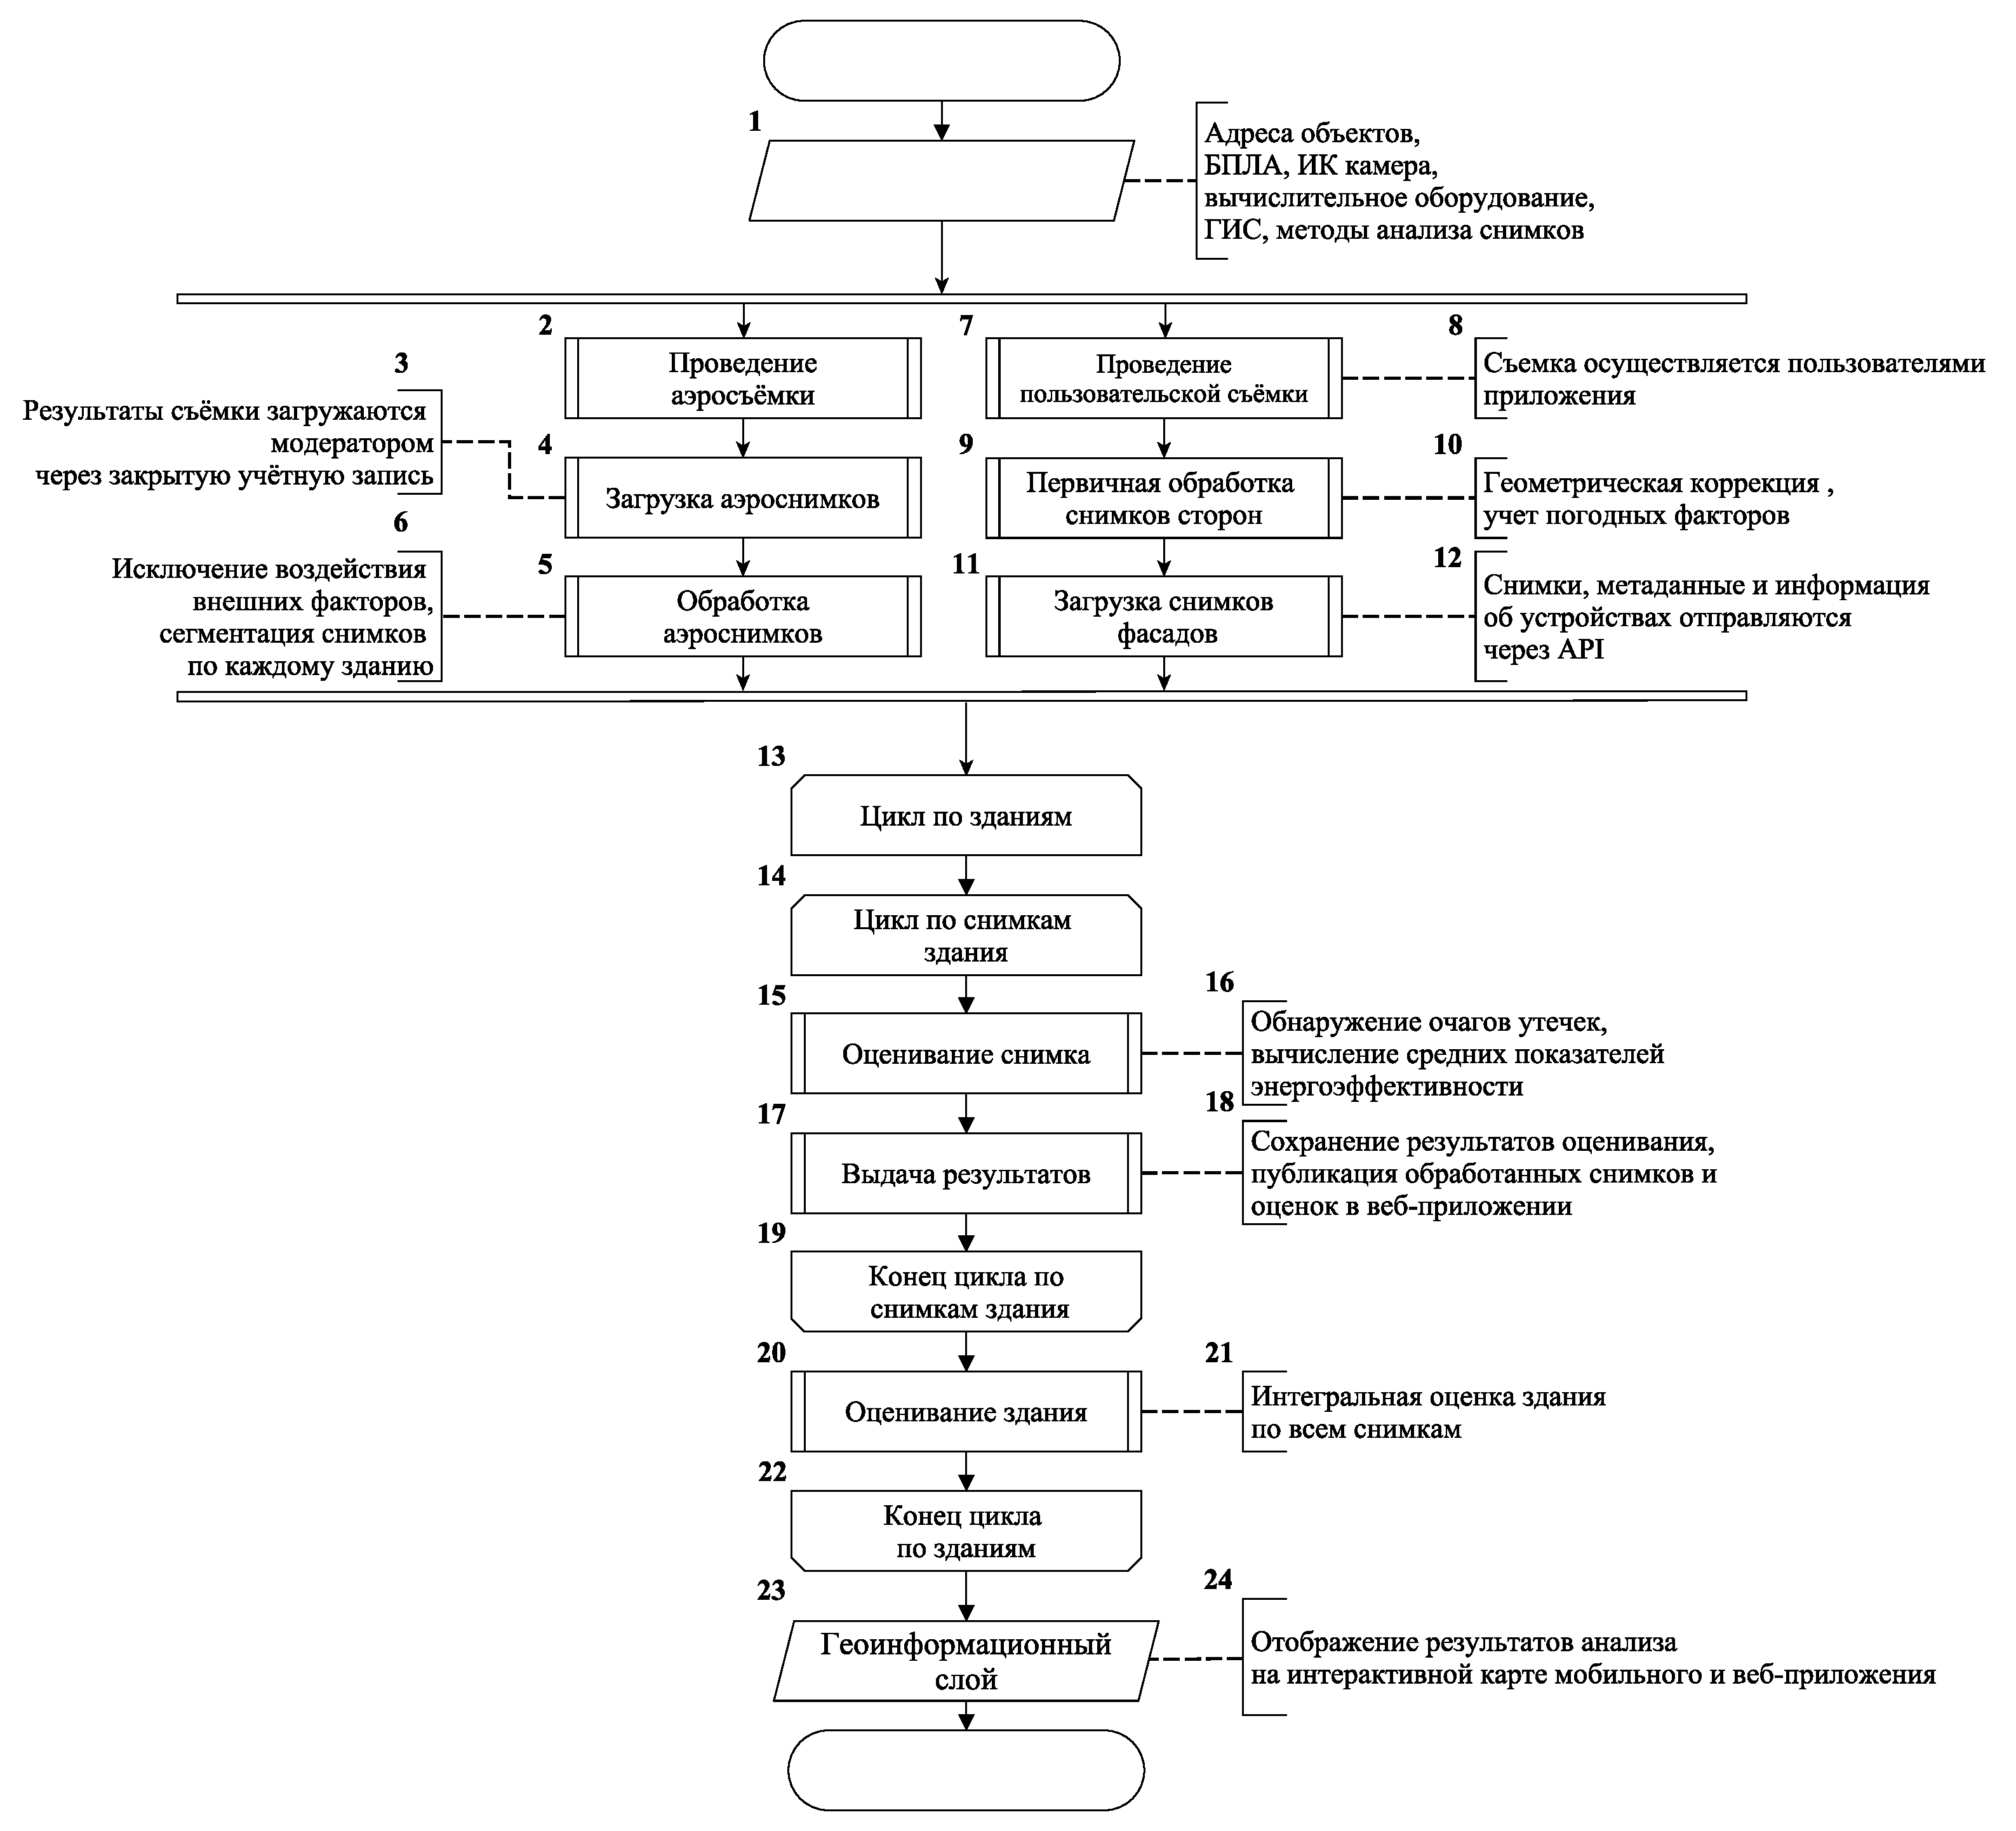
\includegraphics[width=0.9\textwidth]{images/am/am0_after}
      \caption{Алгоритм исследования утечек в жилых зданиях (для предлагаемого решения)}
      \label{am:after:common}
    \end{figure}

    \begin{figure}[t!]
      \centering
      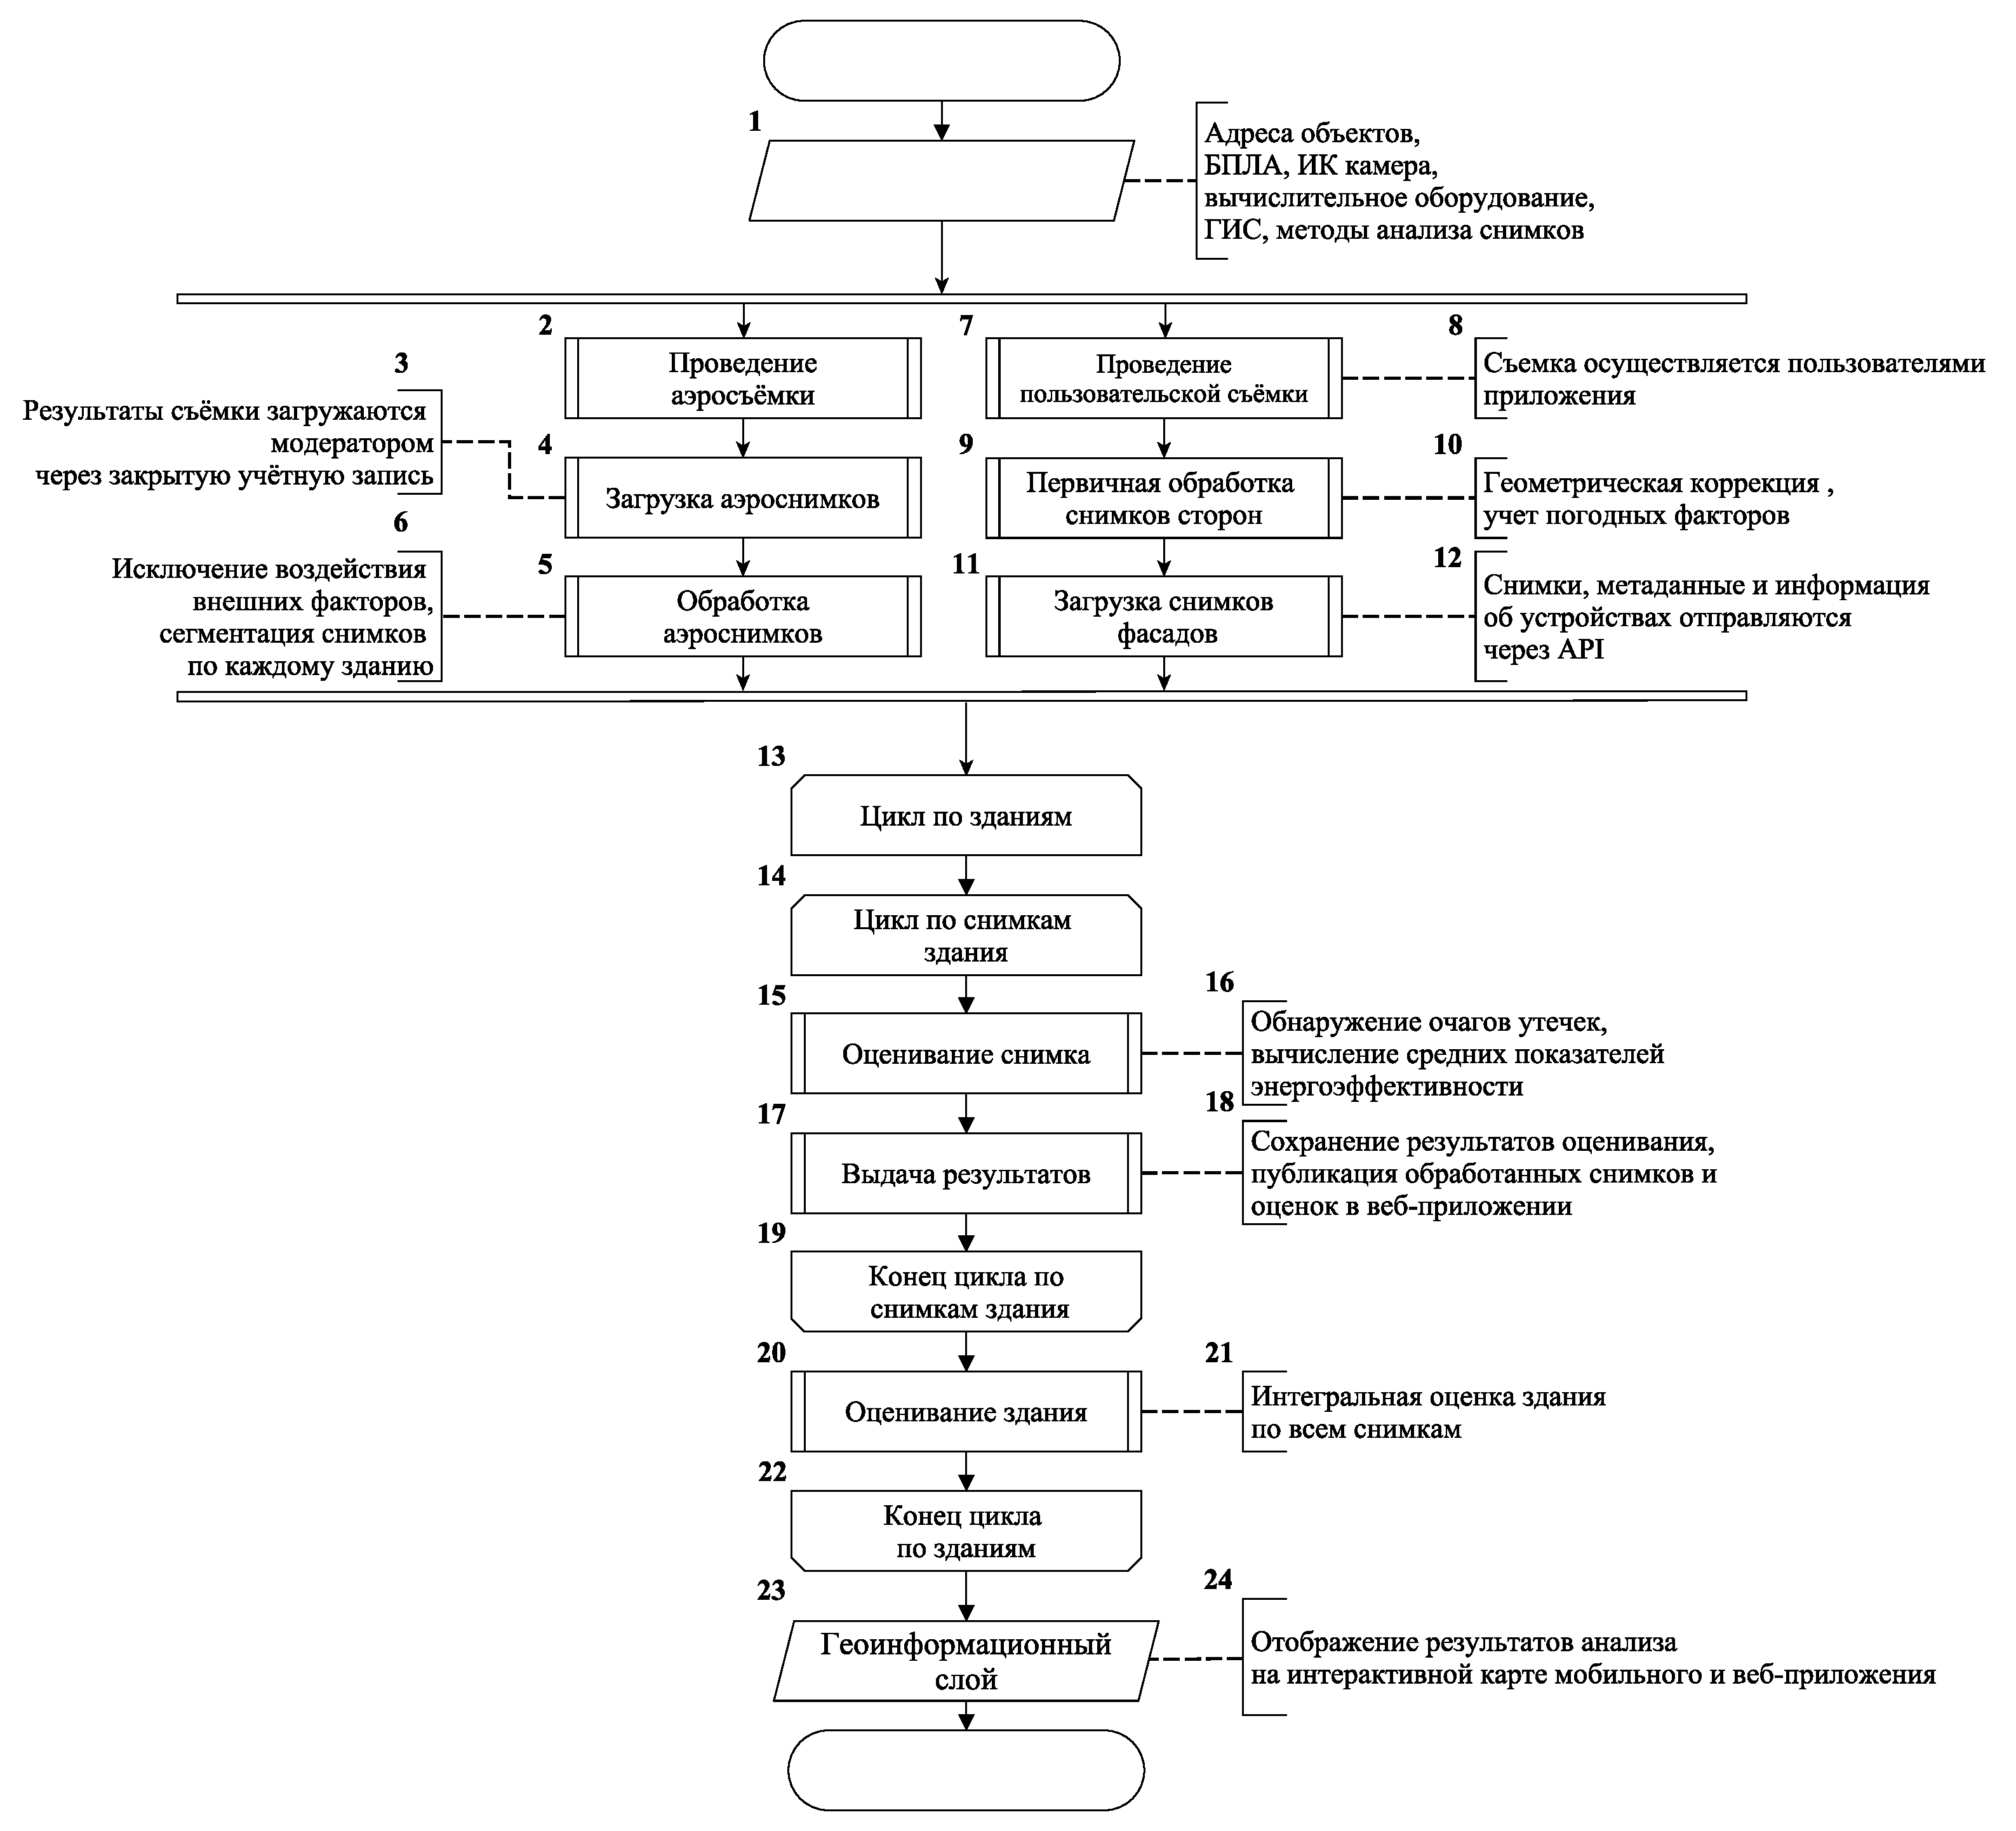
\includegraphics[width=0.9\textwidth]{images/am/am0_after}
      \caption{Общий алгоритм получения оценок энергоэффективности (для предлагаемого решения)}
      \label{am:after:integral}
    \end{figure}

\pagebreak

\par
	После внедрения новых подсистем процедура получения пользователем информации из системы также претерпевает изменения. Сравнение алгоритмов работы с системой до изменений (рисунок \ref{am:before:common}) и после них (рисунок \ref{am:after:common}) позволяет их выделить.

	\begin{figure}[t!]
      \centering
      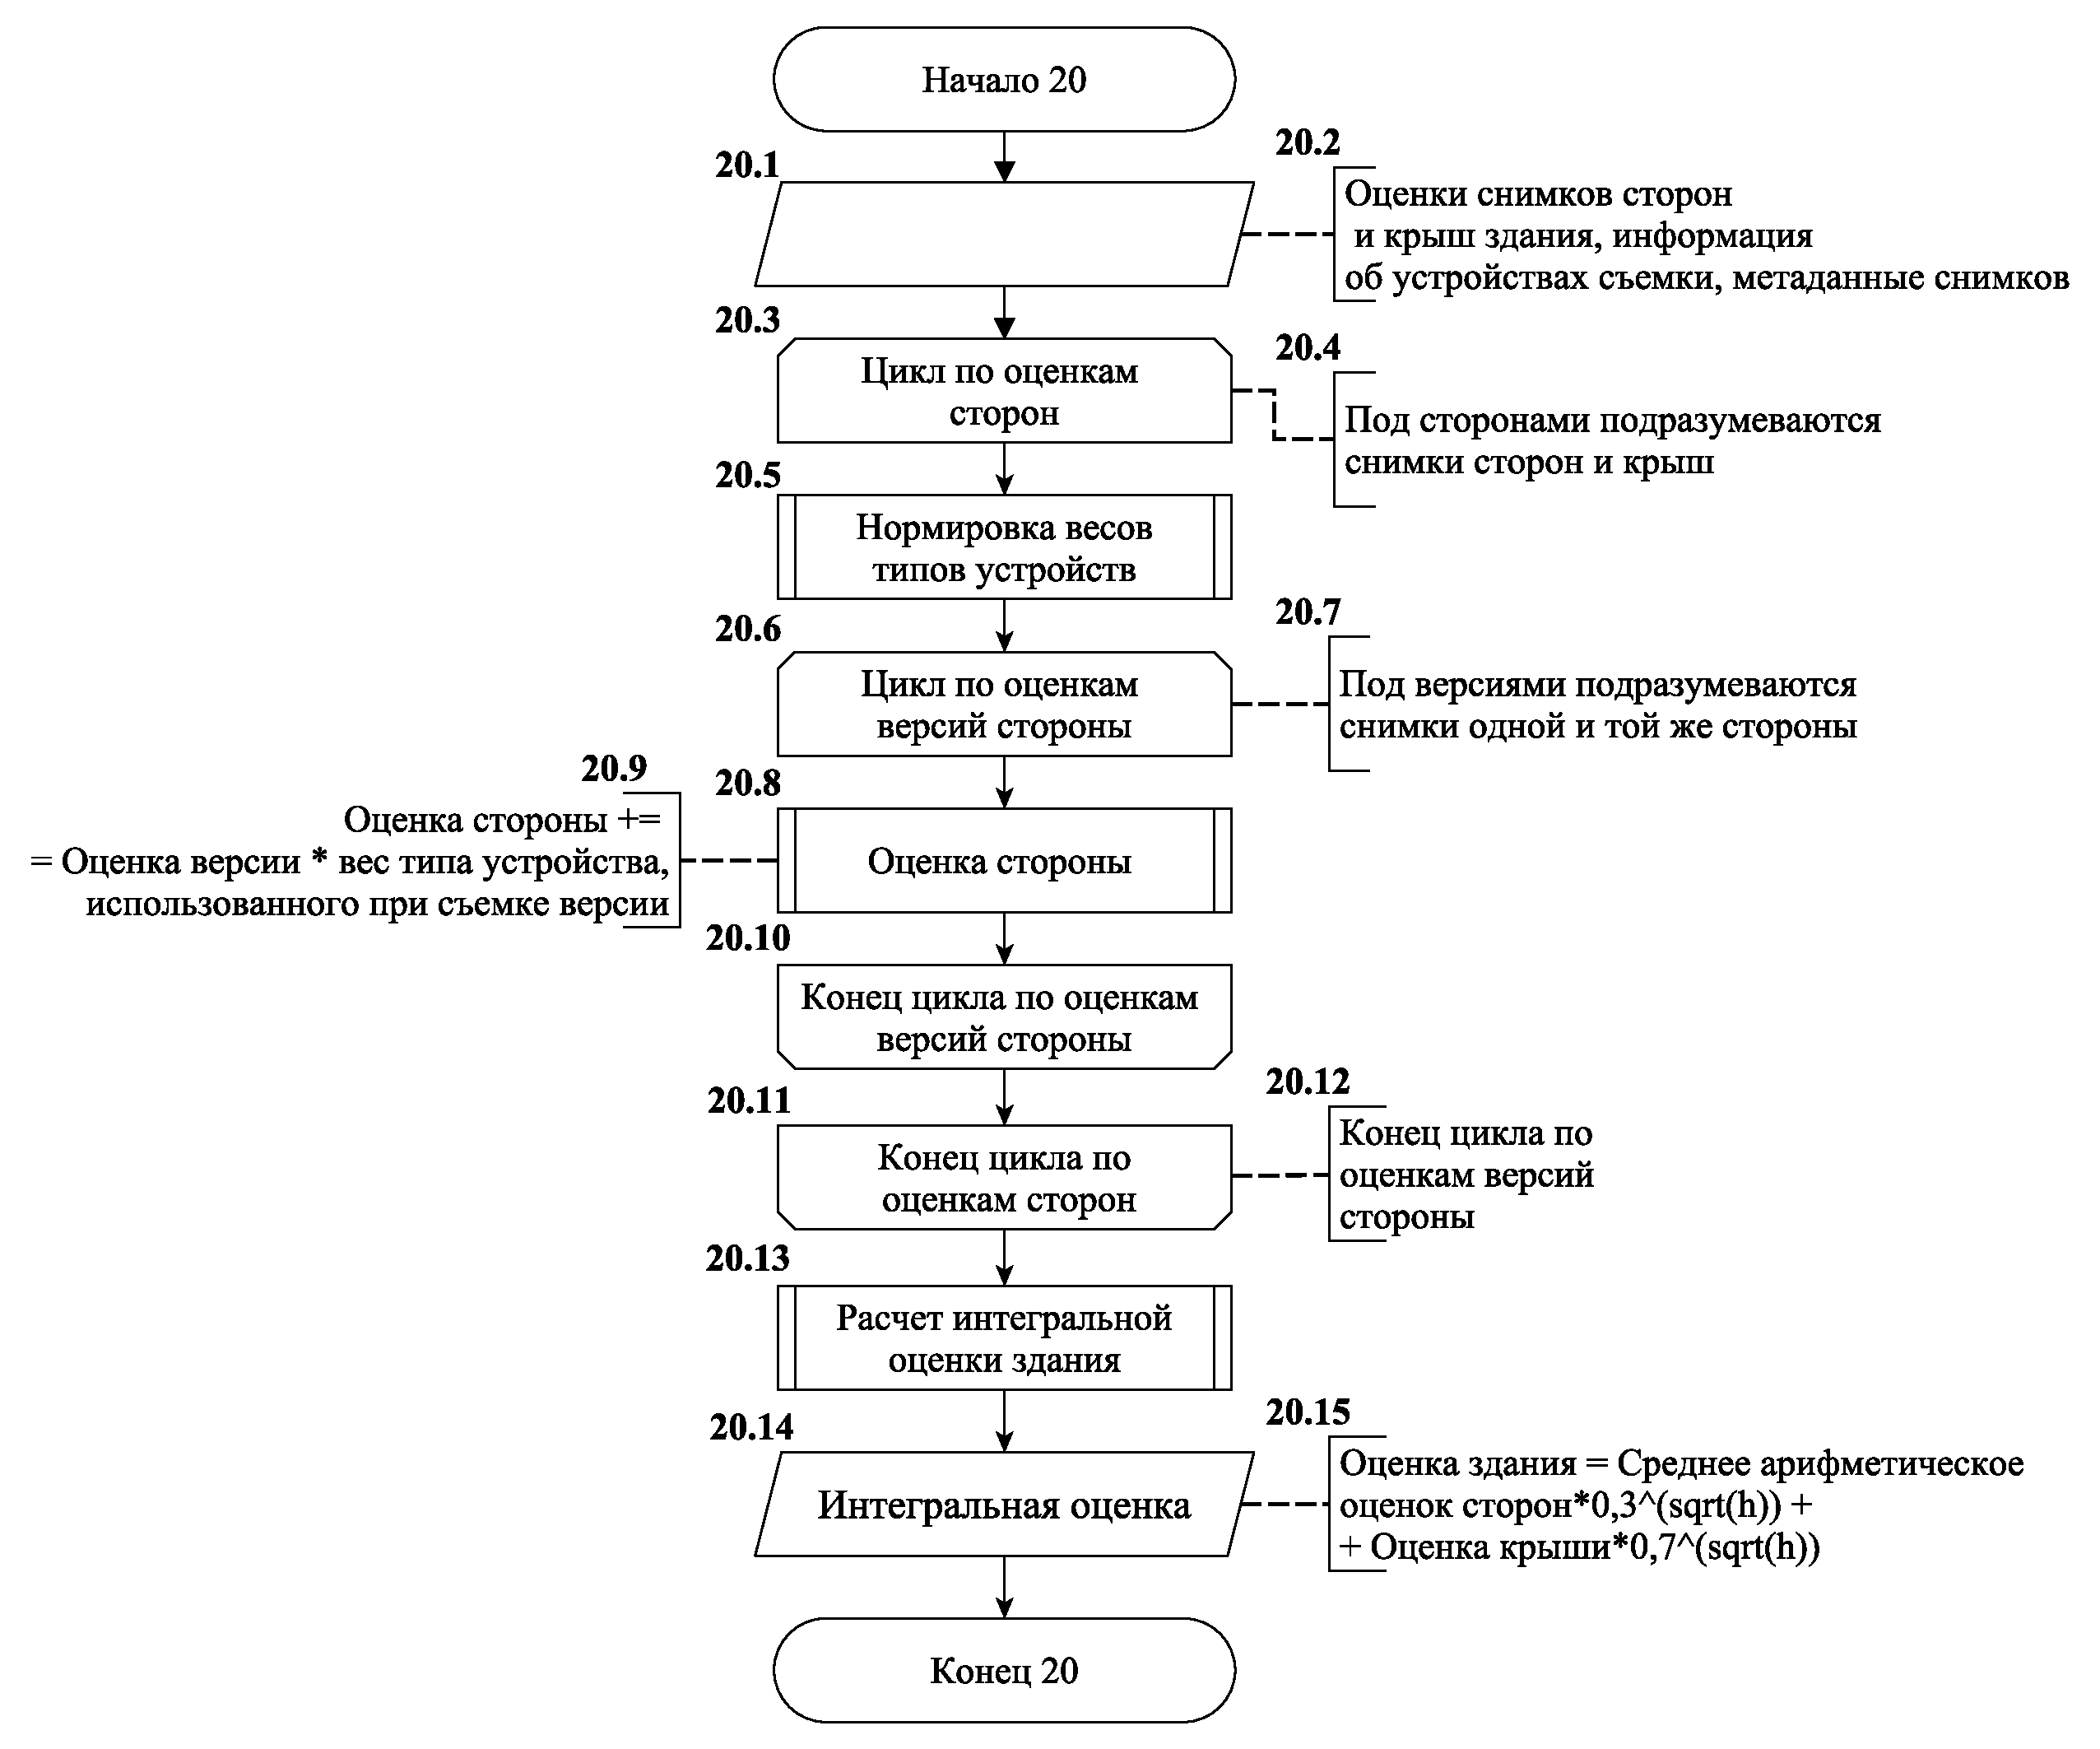
\includegraphics[width=0.9\textwidth]{images/am/am02_after}
      \caption{Алгоритм использования системы в целях получения информации об энергоэффективности жилых зданий (для предлагаемого решения)}
      \label{am:after:common}
    \end{figure}

\pagebreak

\section{Результаты и выводы по главе 2}
\label{sec:models:summary}

\par
	На основе информации, полученных в результате изучения материалов, приведённых в главе 1, были построены модели прототипа и предлагаемого решения. В целях выделения специфики между существующей системой и предлагаемым решением представлена структурно-функциональная модель и алгоритмы работы с подсистемами прототипа и новой системы.

	Благодаря тому, что моделирование проводилось как для системы в целом, так и для разрабатываемого программного интерфейса, можно получить представление о том, как изменяются отдельные компоненты системы, как взаимодействуют информационные потоки смежных с API подсистем и внешней среды всей системы анализа тепловых утечек. Взаимосвязь между системой в целом и её подсистемами показана в концептуальной, системно-структурной и структурно-функциональной моделях.

	Алгоритмы, представленные в разделе \ref{sec:models:algo}, имеют целью продемонстрировать ключевые изменения в работе компонентов системы, а также в работе пользователей с системой.

	Таким образом, становится возможным формулирование конкретного списка требований, которым должны удовлетворять все подсистемы в новом решении на этапе проектирования и задач, которые необходимо выполнить при реализации нового решения в рамках данной работы.


\chapter{Проектирование предлагаемого решения}

\section{Внешнее проектирование}

\par
	В результате внешнего проектирования было получено техническое задание по ГОСТ 34.602-89 на разработку программного интерфейса (API) искомой системы, приведенное в приложении *.

\section{Внутреннее проектирование}

\par

	На основе требований, выдвинутых в техническом задании и результатов моделирования, приведённых в главе \ref{chap:models} проведено внутреннее проектирование API САТУ.

	Согласно требованиям, API САТУ взаимодействует с клиентскими приложениями через Интернет. В этой связи разумно использовать инструменты, ориентированные на работу в Web.

	Для разработки программного интерфейса системы анализа тепловых утечек в городских зданиях был выбран сценарный язык программирования PHP, поддерживающий концепцию ООП, поддерживающий концепцию объектно-ориентированного программирования. Основная причина выбора этого языка - распространённость его использования в web-проектах, в том числе для web-API, в силу наличия большого количества встроенных библиотек, ориентированных на разработку web-проектов.


\par

	Проектирование API выполнено на основе шаблона {MVC (Model-View-Controller)}, который подразумевает деление программного кода на 3 отдельных компонента: \textit{модель} (отвечает за обработку данных), \textit{представление} (отвечает за получение и отправление данных) и \textit{контроллер} (содержит управляющую логику, использует модели и представления). MVC позволяет сделать независимым код, отвечающий за работу с данными от кода, отвечающего за приём и отправку запросов [*].
	
	В качестве подхода к проектированию взаимодействия клиентских приложений и компонентов системы, работающих на сервере, была взят архитектурный стиль REST. Ограничения, определённые в REST, позволяют создавать масштабируемые и унифицированные программные интерфейсы [*]. REST использует в качестве протокола прикладного уровня HTTP.
	
	Стандарт, который использует API для форматирования сообщений - JSON. Формат JSON подходит для передачи сообщений со сложной структурой и уместен при обмене данными между клиентскими приложениями и сервером.
	
	Согласно требованиям в техническом задании (приложение \ref{app-tz}), а также алгоритму итогового оценивания энергоэффективности (раздел \ref{sec:models:algo:after}), API взаимодействует с данными САТУ с помощью СУБД, а именно обеспечивает загрузку и выгрузку снимков зданий. Таким образом, API необходим доступ к базе данных САТУ. Для инженерной реализации была спроектирована та часть базы данных САТУ, которая будет задействована в работе API. \\

	Проектирование базы данных выполнялось на основе ER-модели (“сущность-связь”). Соответствующая ER-диаграмма представлена на рисунке \ref{erd:1} и включает в себя основные сущности:

	\textbf{Пользователь} (\texttt{user}) - хранит идентификационные данные пользователей, их контакты, а также некоторые технические данные для системы аутентификации.

	\textbf{Здание} (\texttt{building}) - хранит данные из ГИС, необходимые для САТУ (в том числе результаты оценивания). Необходим для прикрепления к конкретным зданиям серий снимков.

	\textbf{Снимок} (\texttt{snapshot}) - хранит данные, полученные пользователями с различных устройств, в том числе ИК изображения (в двоичном представлении), координаты съёмки, а также данные, собранные со вспомогательных датчиков в момент съёмки здания устройством.

	\textbf{Серия снимков} (\texttt{snapshot\_series}) - используется для объединения снимков зданий, выполненных конкретным пользователем с помощью конкретного ИК устройства за определённый интервал времени. Это необходимо для правильного хранения версий снимков здания за счёт логических ограничений в структуре базы данных. 

	\textbf{ИК устройство} (\texttt{ir\_device}) - позволяет централизованно хранить всю техническую информацию об устройствах съёмки (тепловизорах). Таким образом, у клиентов нет необходимости отсылать эти данные после каждой серии съёмки.

	\textbf{Приложение} (\texttt{application}) - хранит идентификационные данные клиентских приложений, сведения об ограничениях доступа к функциям API и дополнительные сведения о его конфигурации.

	\textbf{Ключ доступа} (\texttt{token}) - предназначен для хранения ключей доступа, привязанных к приложению, а также информации об этих ключах: тип доступа(ограниченный/неограниченный), статус(активен/неактивен). Хранение токенов необходимо для того, чтобы исключить дублирование при генерации новых.

	\textbf{Журналы} (\texttt{log\_user}, \texttt{log\_application}) - используются для фиксирования некоторых действий пользователей и приложений в целях отладки клиентских программ.

	\pagebreak

	\begin{landscape}

		\begin{figure}[t!]
		      \centering
		      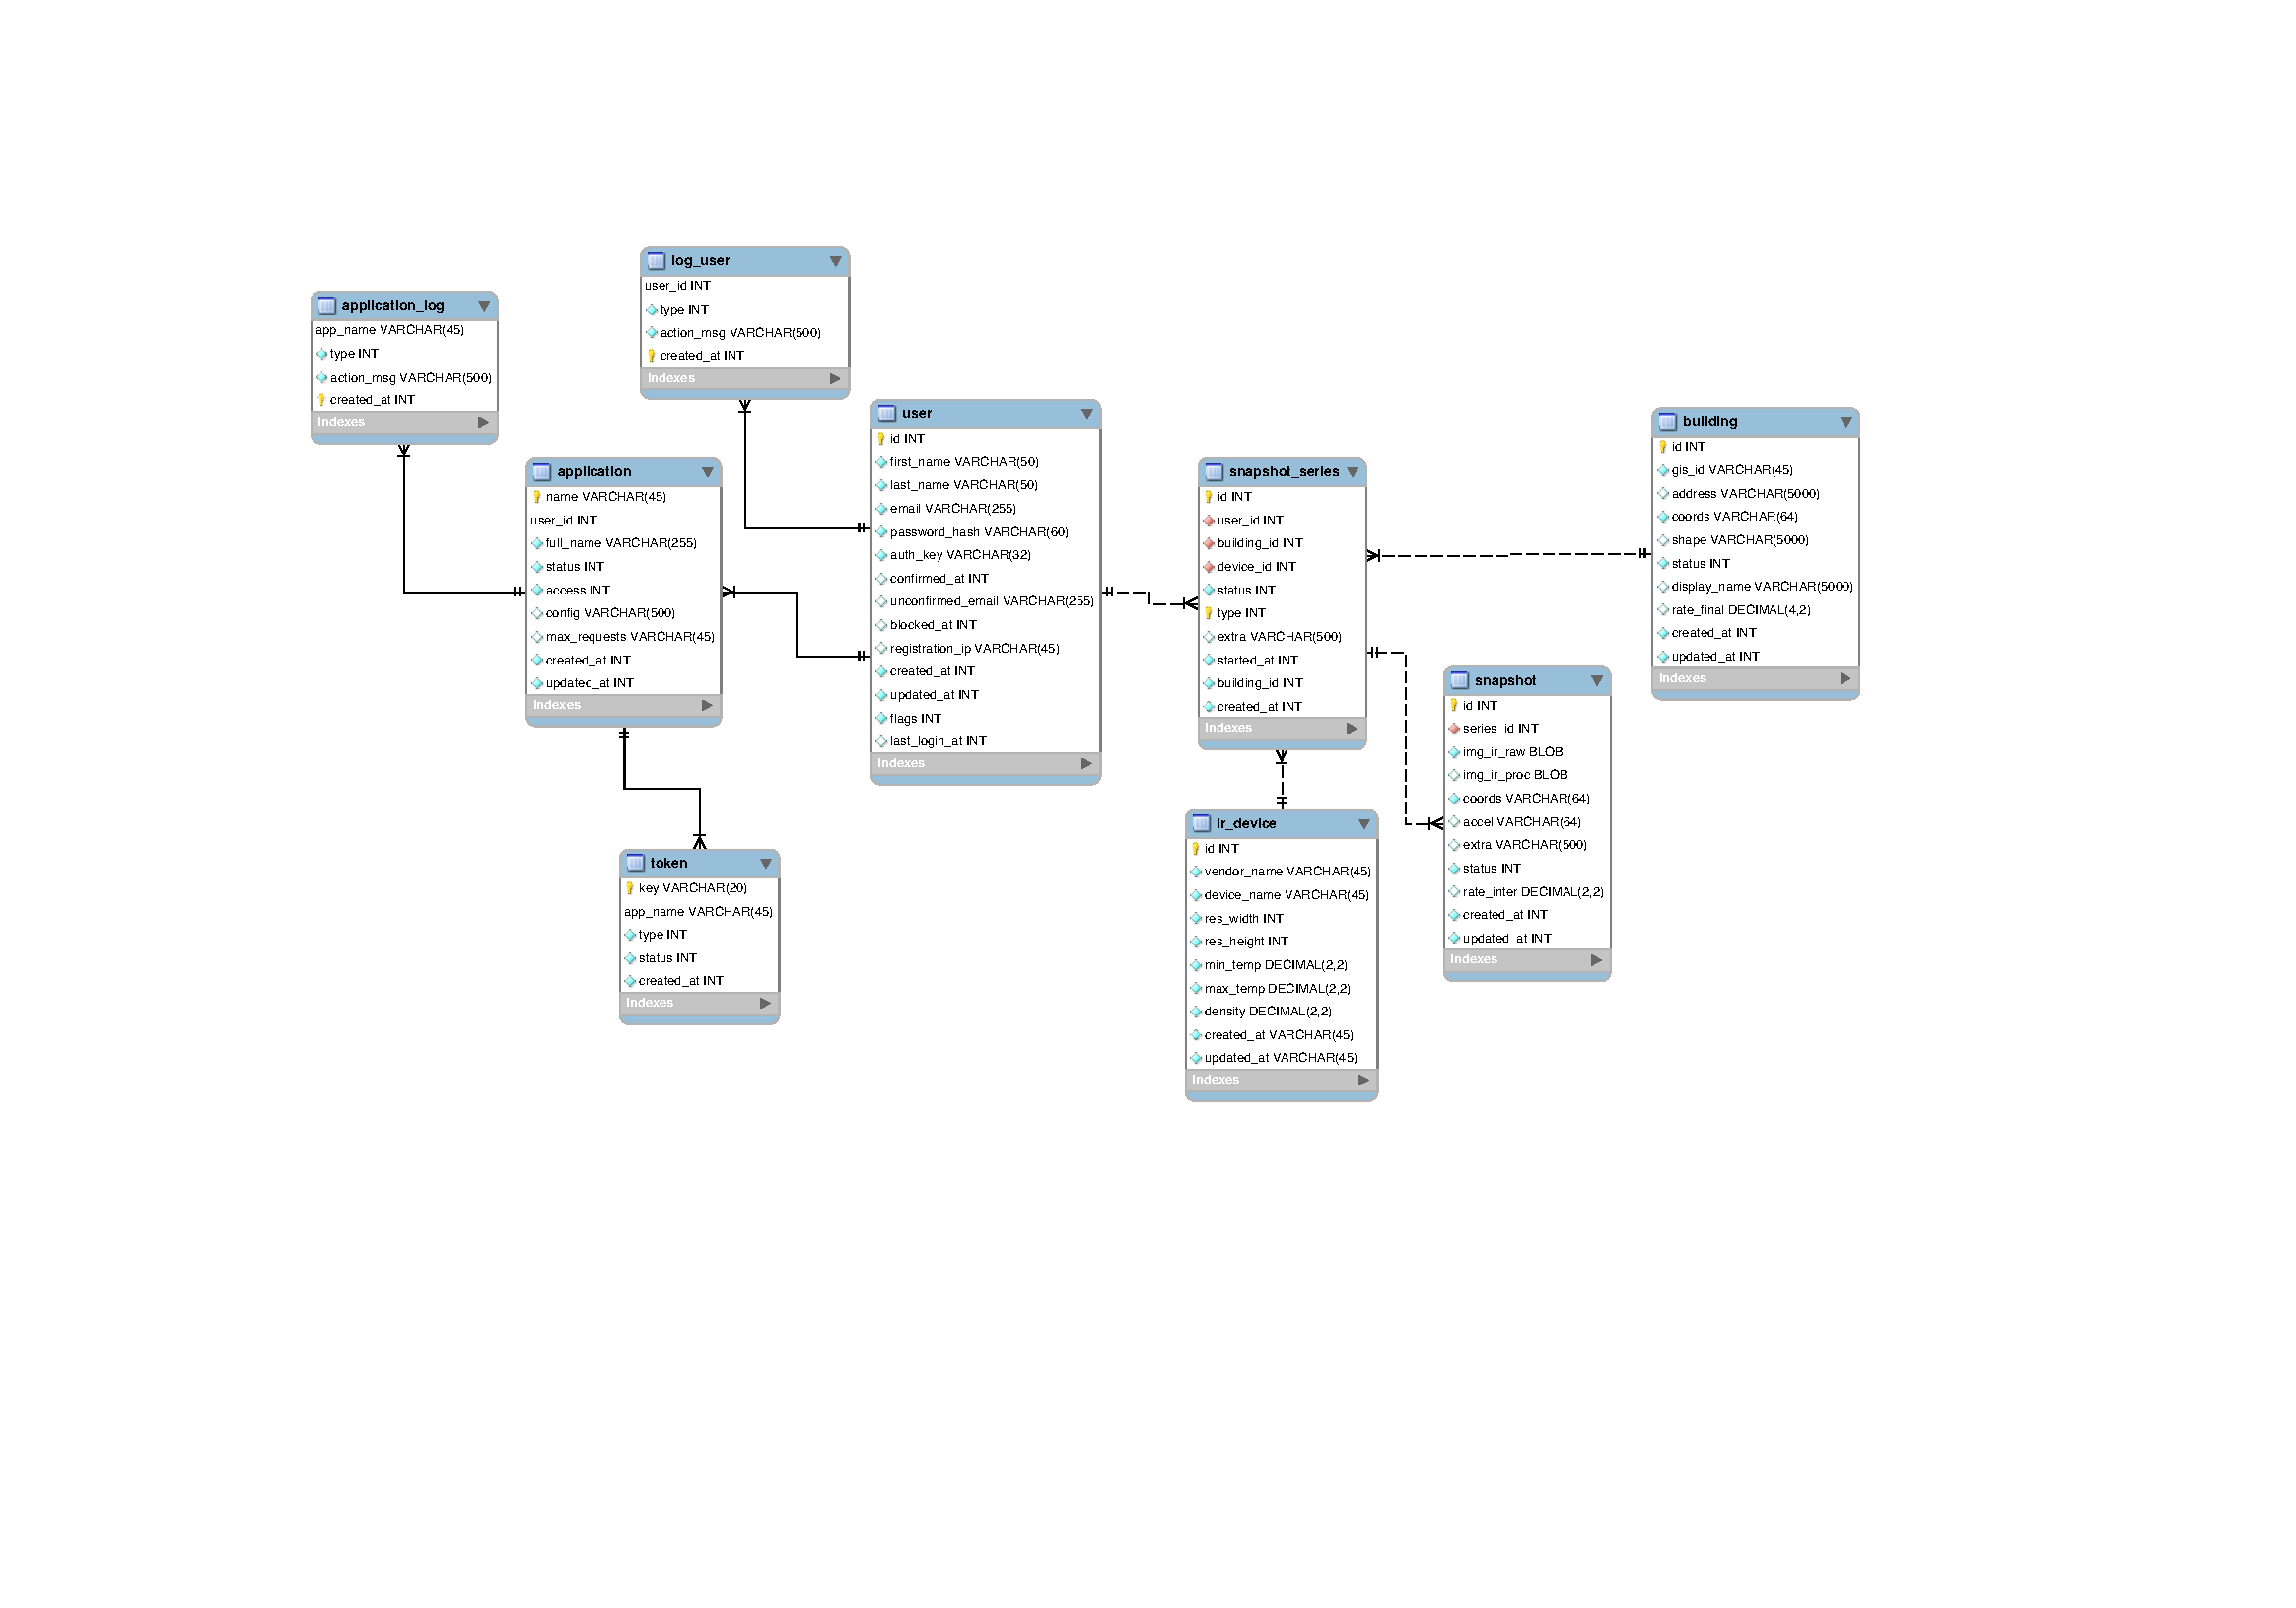
\includegraphics[width=1.3\textwidth]{images/erd/1}
		      \caption{Фрагмент схемы базы данных САТУ, используемой программным интерфейсом}
		      \label{erd:1}
		\end{figure}

	\end{landscape}

	\pagebreak

	На основе полученной схемы базы данных была спроектирована архитектура взаимодействия клиентских приложений с API путём изображения ресурсов, предоставляемых API и ссылок на эти ресурсы. Схемы, получаемые в результате проектирования, полезны при написании программного кода, когда точно сформулированы запросы, их параметры, определены необходимые для работы функций классы. Кроме того, эти схемы можно использовать при создании руководства программиста, поскольку в основном описывает набор доступных запросов, входные и выходные данные, их формат и структуру.

	При проектировании REST API используют диаграммы классов [ссылка]. Каждый ресурс характеризуется названием, идентификатором (URI), соответствующим HTTP-методом и набором параметров. Ресурсы на диаграмме изображены скругленными прямоугольниками. В качестве описателей входных и выходных данных ресурсов используют классы (выделены прямоугольной рамкой). Проектирование выполнено с помощью программного пакета Visual Paradigm 14.1, предусматривающего функцию генерации каркаса программного кода на основе построенных моделей.

	На рисунке \ref{uml:1} представлена диаграмма классов, описывающая набор ресурсов, специфичных для САТУ. Классы и ресурсы, относящиеся к авторизации пользователей и приложений, в данной диаграмме опущены.

	\pagebreak

	\begin{landscape}

		\begin{figure}[t!]
		      \centering
		      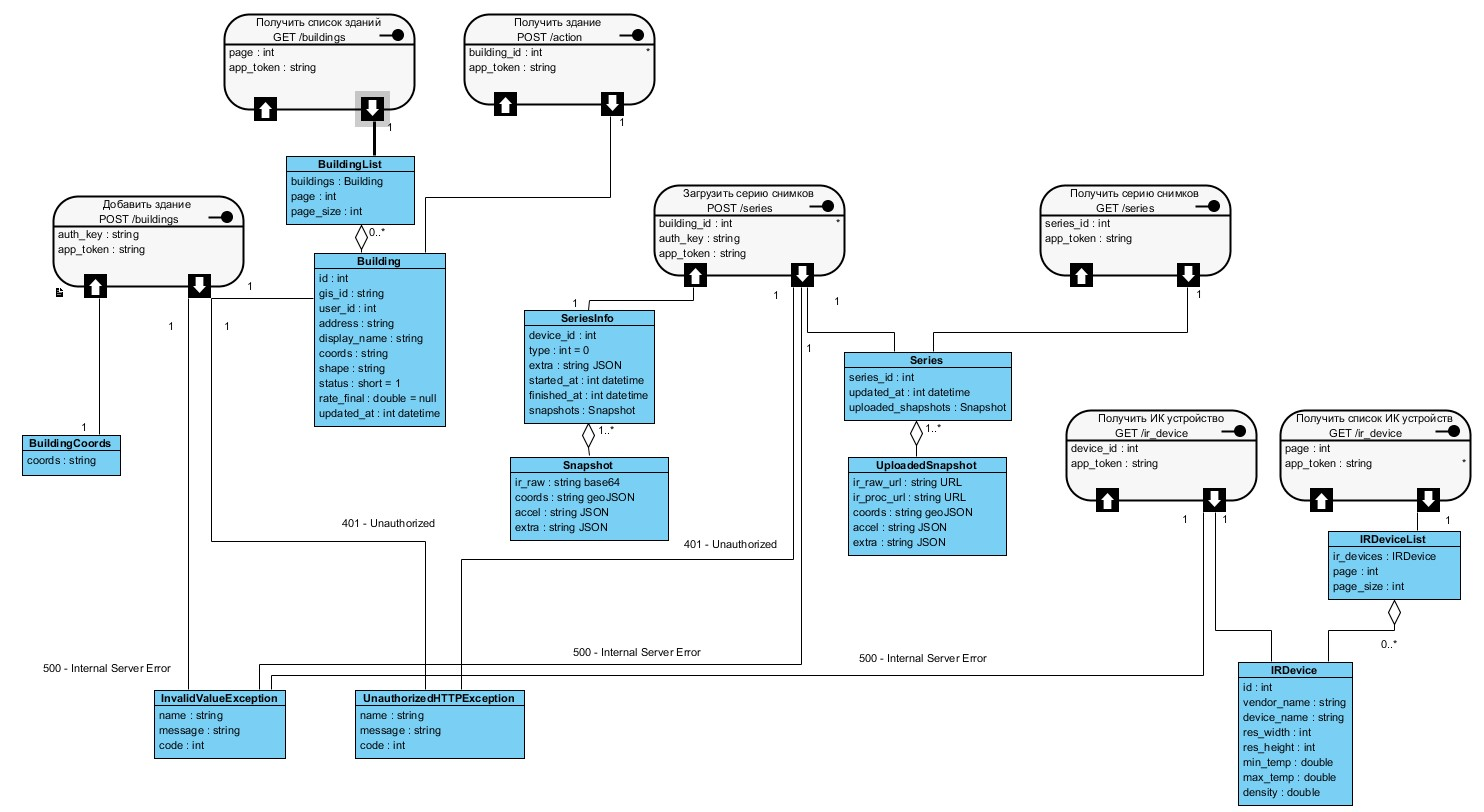
\includegraphics[width=1.3\textwidth]{images/uml/1}
		      \caption{Фрагмент диаграммы классов, описывающей структуру основной части API САТУ}
		      \label{uml:1}
		\end{figure}

	\end{landscape}

	\pagebreak

	Атрибуты некоторых классов в представленной диаграмме во многом совпадают с атрибутами сущностей в ER-диаграмме. Тем не менее, атрибуты классов показывают, что должен включать в себя тот или иной HTTP-запрос к ресурсу. При обращении к нему клиентская программа должна учитывать правильность соблюдения не только типов передаваемых данных, но и структуры отправляемого запроса.

	Некоторые классы связаны между собой отношением агрегации. Например, чтобы загрузить снимки какого-либо здания в систему, требуется передать данные о съёмке (класс \texttt{SeriesInfo}): идентификатор ИК устройства (\texttt{device\_id}), тип съёмки (\texttt{type}), а также несколько снимков (\texttt{snapshots}), где каждый снимок (класс \texttt{Snapshot}) описан четырьмя атрибутами: изображение, закодированное в формате base64, координаты снимка, данные встроенного акселерометра в формате JSON (\texttt{accel}) и т. п.

	В данной диаграмме обозначены классы \texttt{InvalidValueException}, \texttt{UnauthorizedHTTPException}, которые используются для оповещения клиентов об ошибках при передаче невалидных данных и при некорректной аутентификации/авторизации. HTTP-ответы, содержащие сведения об ошибке, API помечает соответствующим статусом. В соответствии с REST [ссылка], коды ошибок необходимо использовать по назначению, когда это возможно.

	\pagebreak

\section{Результаты и выводы по главе 3}

\par
	
	На основе полученных на этапе моделирования результатов сформулированы требования к разрабатываемому программному интерфейсу, определены программные средства и архитектурные принципы, которые легли в основу внутреннего проекта. Таким образом, были достигнуты следующие результаты:

	\begin{itemize}
		\item составлено Техническое задание на разработку системы (приложение \ref{app-tz});
		\item определён набор программных средств и инструментов для создания системы;
		\item разработаны решения по программной архитектуре системы.
	\end{itemize}


\chapter{Инженерная реализация}

\section{Описание реализации}

Выбранные архитектурные принципы, стандарты и инструменты, утверждённые на этапе проектирования, поддерживаются программной платформой Yii 2 Framework. Данная платформа ориентирована на ускорение процесса разработки web-проектов, в том числе API по принципу REST, за счёт наличия большого числа программных модулей и автоматической генерации программного кода на основе схем баз данных. В результате внутреннего проектирования предлагаемого решения выяснилось, что эта платформа является наиболее подходящей.

\subsection{Примеры запросов и ответов API}

Отправка запросов и получение ответов выполнялось с помощью среды тестирования и отладки API Postman. Каждое сообщение содержит заголовок и тело, содержимое которых определяется ресурсом в соответствии с диаграммой на рисунке \ref{uml:1}.
	
	Для отправки запроса на добавление здания необходимо передать API запрос, аналогичный представленному на рисунке \ref{query:buildings_post_to}. При этом возможны два сценария: здание успешно добавлено (рисунок \ref{query:buildings_post_from}), здание уже существует (рисунок \ref{query:buildings_post_err_exists}).

	\pagebreak

	\begin{figure}[t!]
		\centering
		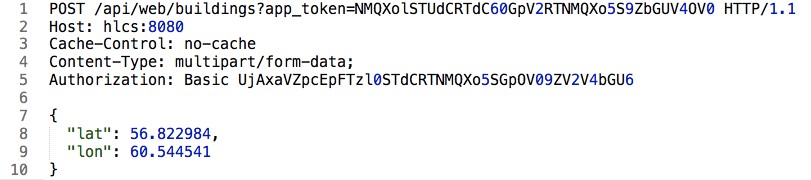
\includegraphics[width=0.8\textwidth]{images/queries/buildings_post_to}
		\caption{Пример запроса на добавление здания в САТУ}
		\label{query:buildings_post_to}
	\end{figure}

	\begin{figure}[t!]
		\centering
		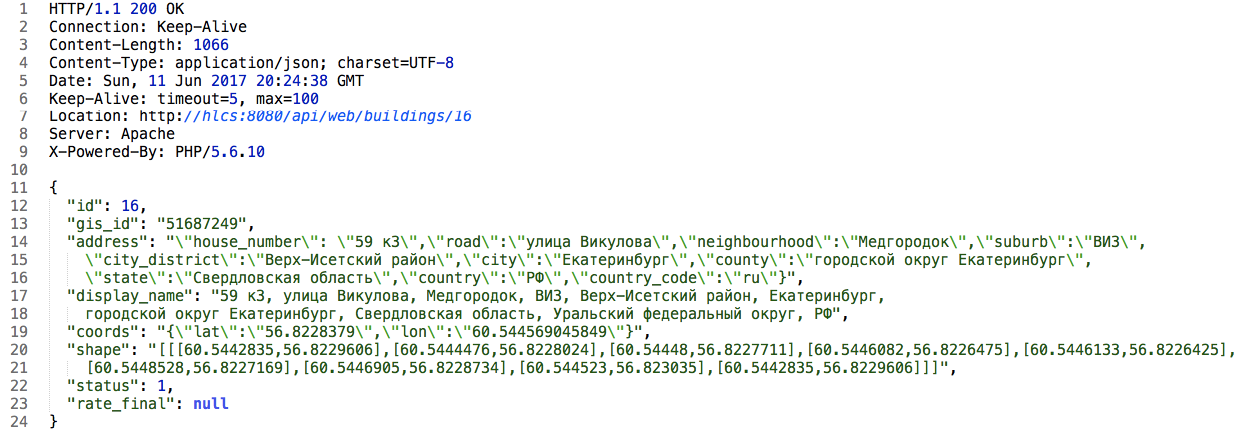
\includegraphics[width=1\textwidth]{images/queries/buildings_post_from}
		\caption{Успешный ответ к запросу на добавление здания в САТУ}
		\label{query:buildings_post_from}
	\end{figure}

	\begin{figure}[t!]
		\centering
		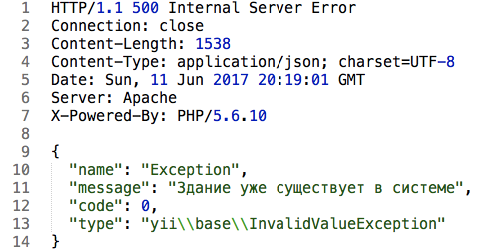
\includegraphics[width=0.5\textwidth]{images/queries/buildings_post_err_exists}
		\caption{Ответ к повторному запросу на добавление того же здания}
		\label{query:buildings_post_err_exists}
	\end{figure}

	Некоторые ресурсы требуют указания ключа авторизации. Если таковые отсутствуют, клиентскому приложению будет возвращён ответ, представленный на рисунке \ref{query:buildings_post_err_unauth}.

	\pagebreak

	\begin{figure}[t!]
		\centering
		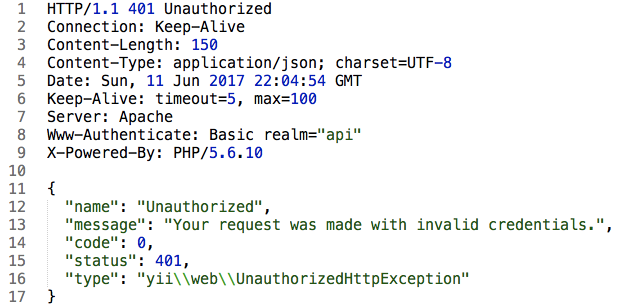
\includegraphics[width=0.6\textwidth]{images/queries/buildings_post_err_unauth}
		\caption{Ответ к запросу без ключа авторизации}
		\label{query:buildings_post_err_unauth}
	\end{figure}

	На рисунке \ref{query:buildings_get_to} приведен пример запроса на получение одной страницы списка всех зданий, соответствующий ответ - на рисунке \ref{query:buildings_get_from}. Из заголовка ответа видно, что объём каждой страницы - 20 элементов. При необходимости получить другую страницу следует изменить параметр \texttt{page}.

	\begin{figure}[t!]
		\centering
		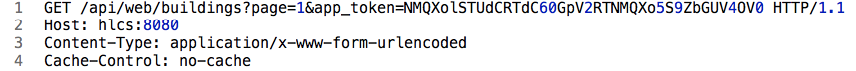
\includegraphics[width=0.9\textwidth]{images/queries/buildings_get_to}
		\caption{Пример запроса на получение списка зданий}
		\label{query:buildings_get_to}
	\end{figure}

	Если требуется получить информацию только по одному конкретному зданию, то к URI предыдущего запроса следует добавить идентификатор здания (рисунок \ref{query:buildings_get_one_to}). В результате от сервера API придёт ответ, аналогичный примеру на рисунке \ref{query:buildings_get_one_from}.

	\pagebreak

	\begin{figure}[t!]
		\centering
		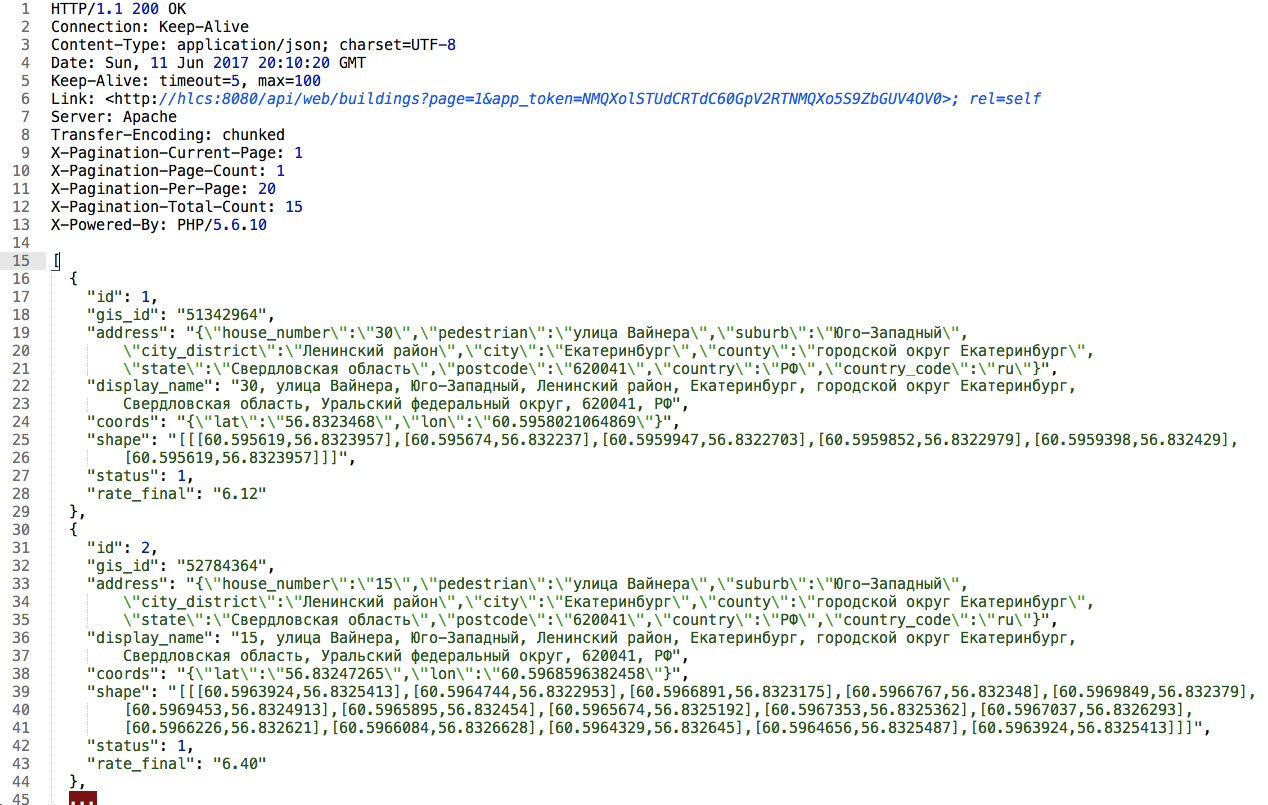
\includegraphics[width=1\textwidth]{images/queries/buildings_get_from}
		\caption{Ответ к запросу на получение списка зданий}
		\label{query:buildings_get_from}
	\end{figure}

	\begin{figure}[t!]
		\centering
		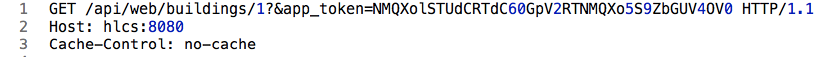
\includegraphics[width=0.9\textwidth]{images/queries/buildings_get_one_to}
		\caption{Пример запроса на получение информации о конкретном здании}
		\label{query:buildings_get_one_to}
	\end{figure}

	\begin{figure}[t!]
		\centering
		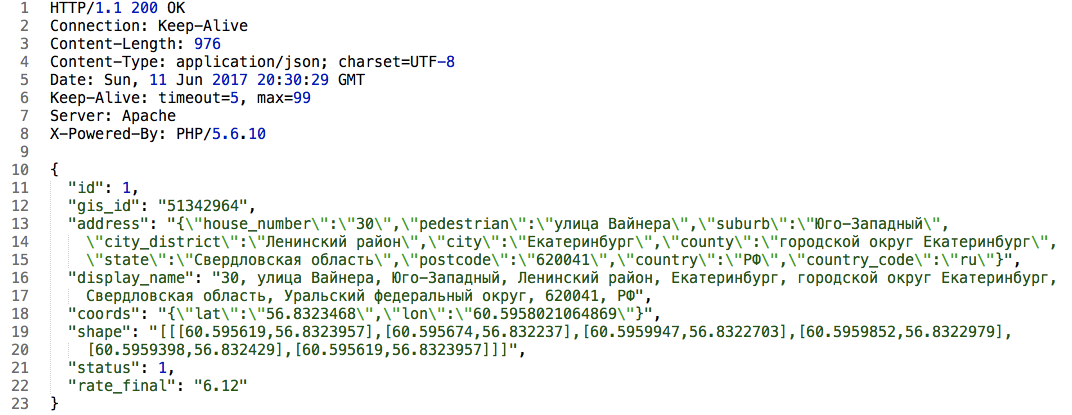
\includegraphics[width=1\textwidth]{images/queries/buildings_get_one_from}
		\caption{Ответ к запросу на получение информации о конкретном здании}
		\label{query:buildings_get_one_from}
	\end{figure}

\subsection{Экранные формы}

	Пользовательский интерфейс прототипа не содержит элементы доступа к функциям системы, предоставляемым API. В качестве альтернативы предлагаемое решение включает в себя реализацию пользовательского web-интерфейса САТУ, работающего как клиентское приложение, использующее API.
 
	Доступ к web-приложению осуществляется через браузер. Доступ к основным страницам осуществляется с помощью главного меню, расположенного в верхней части каждой web-страницы. Главная страница (рисунок \ref{scrshot:main_1}) поделена на две части: панель поиска зданий и интерактивная карта Google Maps. Здания, которые были проанализированы САТУ, выделяются цветом по шкале от красного до зелёного в соответствии с оценкой энергоэффективности.

	\begin{figure}[h!]
		\centering
		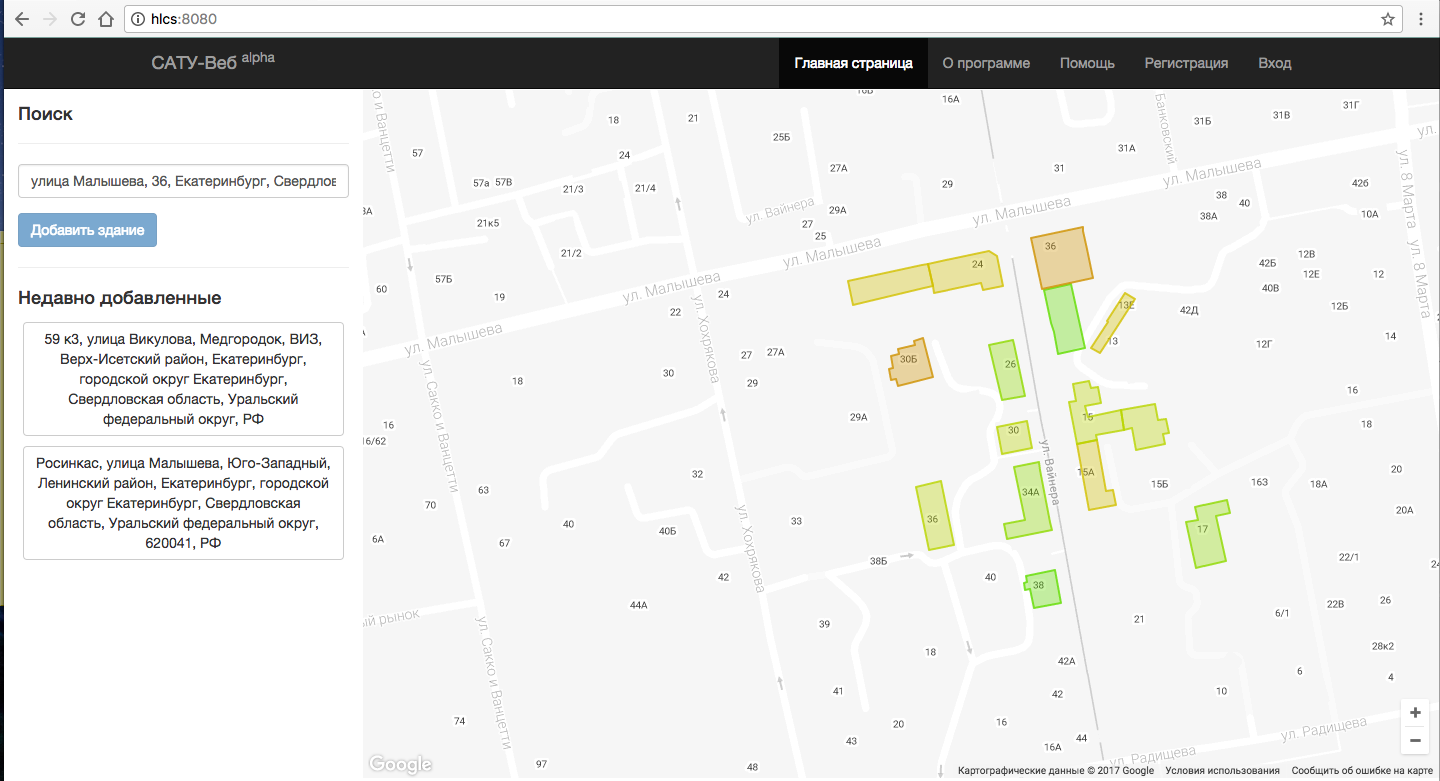
\includegraphics[width=1\textwidth]{images/scrshots/main_1}
		\caption{Главная страница веб-интерфейса САТУ}
		\label{scrshot:main_1}
	\end{figure}

	\pagebreak

	При введении пользователем интересующего адреса в поле поиска формируется выпадающий список (рисунок \ref{scrshot:search_field_1}) с доступными в ГИС адресами зданий.

	\begin{figure}[h!]
		\centering
		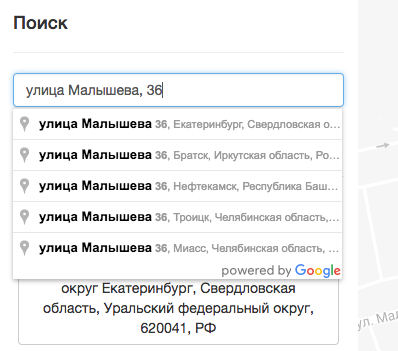
\includegraphics[width=0.5\textwidth]{images/scrshots/search_field_1}
		\caption{Процедура поиска здания в ГИС Google Maps}
		\label{scrshot:search_field_1}
	\end{figure}

	После выбора адреса из списка возможно два варианта поведения: если здание найдено в САТУ, оно отобразится в центре карты; в противном случае здание дополнительно выделяется розовым цветом (рисунок \ref{scrshot:main_new_1}).

	\begin{figure}[t!]
		\centering
		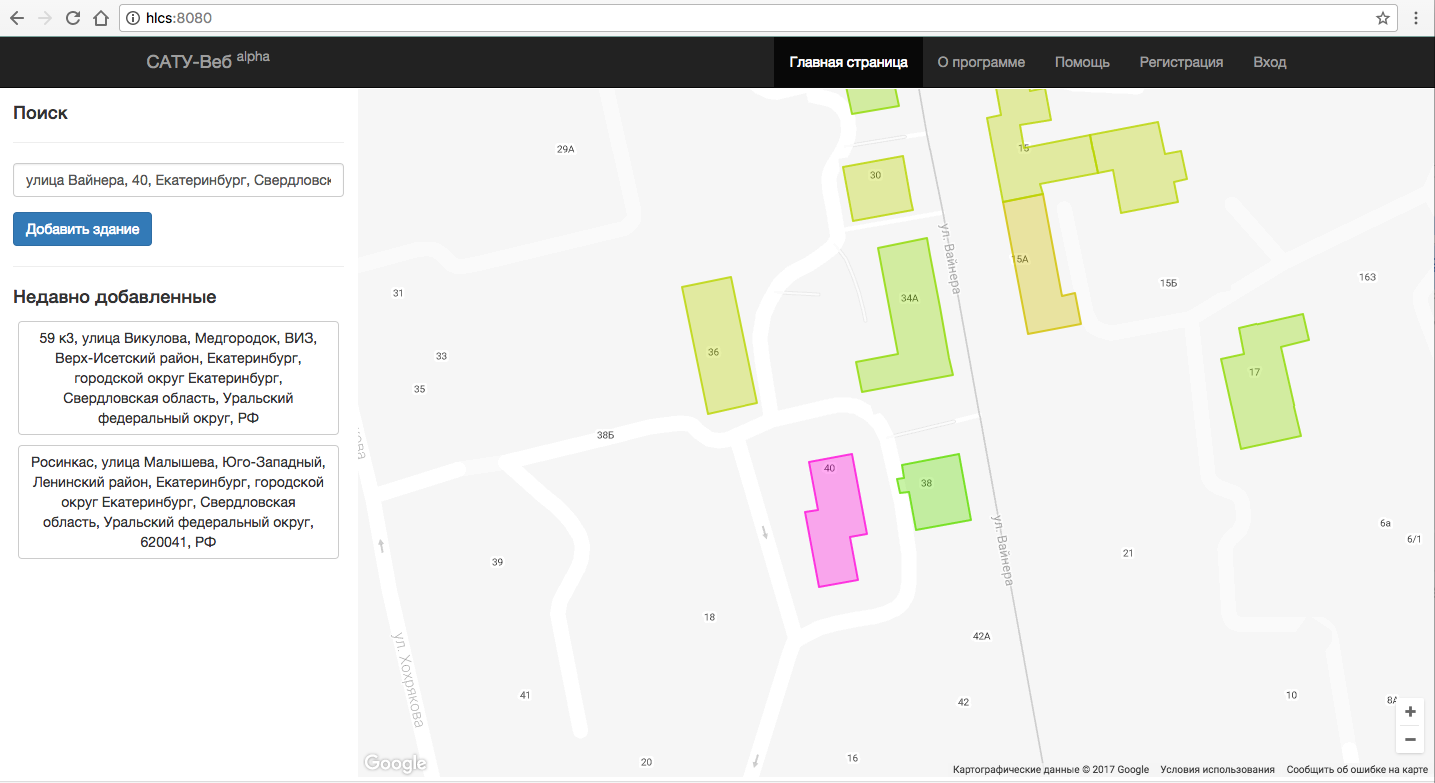
\includegraphics[width=1\textwidth]{images/scrshots/main_new_1}
		\caption{Отображение здания, не обнаруженного в САТУ}
		\label{scrshot:main_new_1}
	\end{figure}


	При нажатии левой кнопкой мыши по подсвеченному зданию на карте рядом с ним отображается всплывающее окно с краткой информацией и ссылкой на страницу с подробными сведениями (рисунок 4.12).

	\begin{figure}[t!]
		\centering
		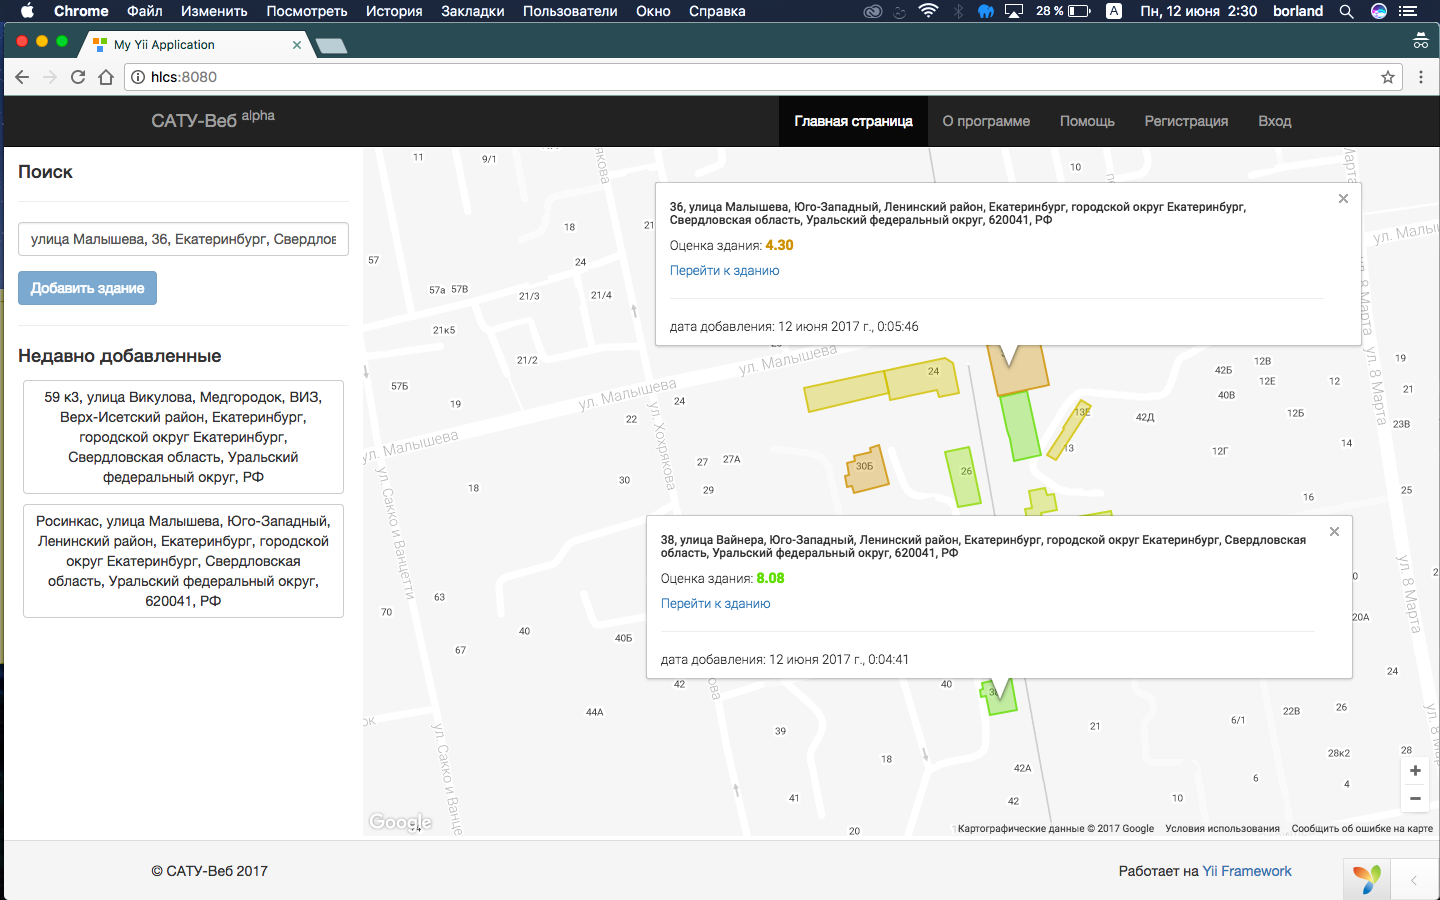
\includegraphics[width=1\textwidth]{images/scrshots/main_selected_1}
		\caption{Взаимодействие с проанализированными зданиями на карте: отображение всплывающих окон}
		\label{scrshot:main_selected_1}
	\end{figure}

	В случае, если здание выделено розовым цветом, в панели поиска становится доступна кнопка “Добавить здание”. При нажатии на неё пользователь перейдёт на страницу “Добавить/изменить здание” (рисунок \ref{scrshot:update_1}). Эта страница позволяет просмотреть историю съёмки здания. При необходимости пользователь может добавить новую серию снимков, нажав на кнопку “Добавить серию снимков”.

	\begin{figure}[t!]
		\centering
		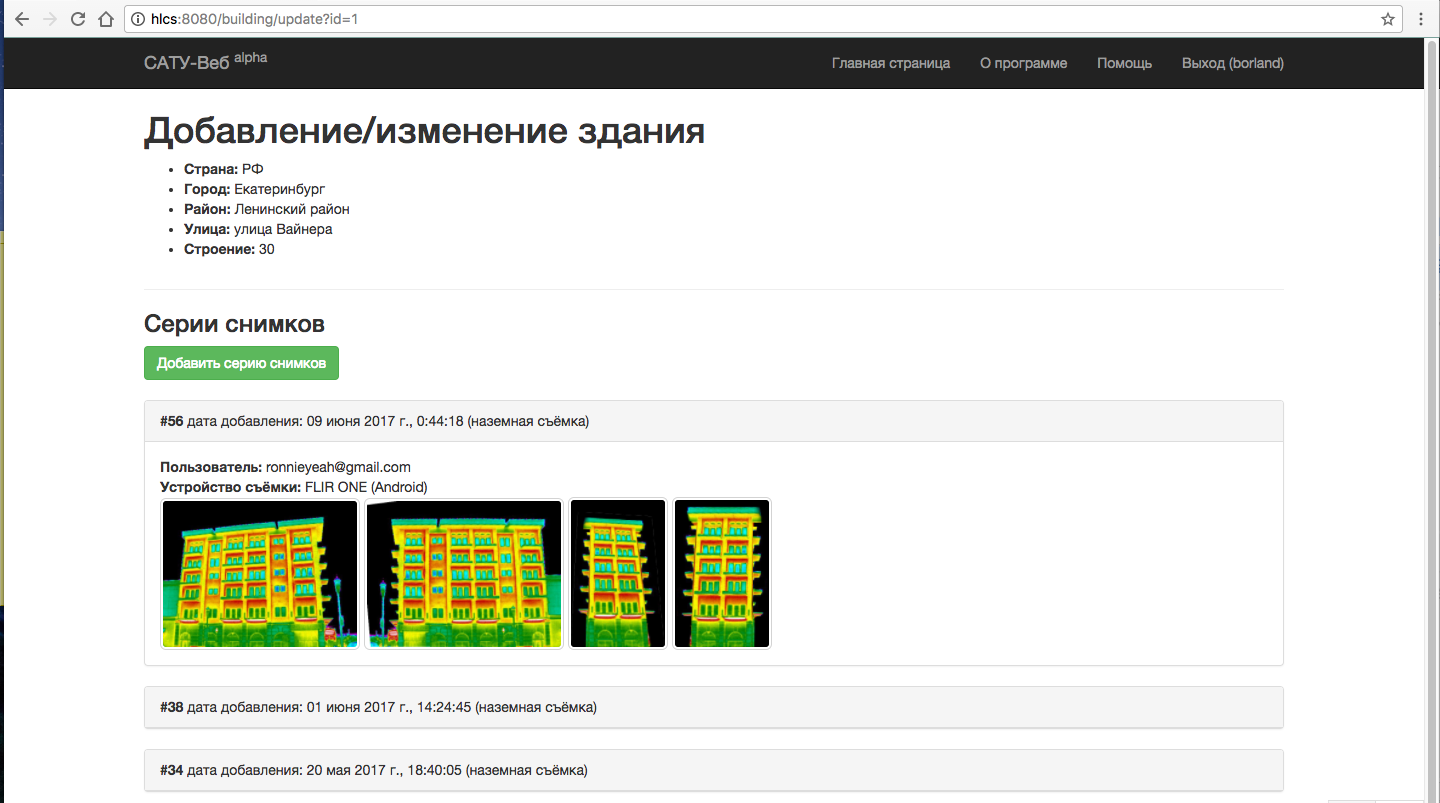
\includegraphics[width=1\textwidth]{images/scrshots/update_1}
		\caption{Форма добавления/изменения здания}
		\label{scrshot:update_1}
	\end{figure}

	Загрузка серии снимков через web-приложение в браузере проходит в два этапа: 

	\begin{itemize}
		\item выбор типа, устройства съёмки, непосредственно загрузка ИК изображений (рисунок \ref{scrshot:add-series_1})
		\item указание дополнительных данных о загруженных снимках (положение камеры) (рисунок \ref{scrshot:add-series_2})
	\end{itemize}

	\begin{figure}[t!]
		\centering
		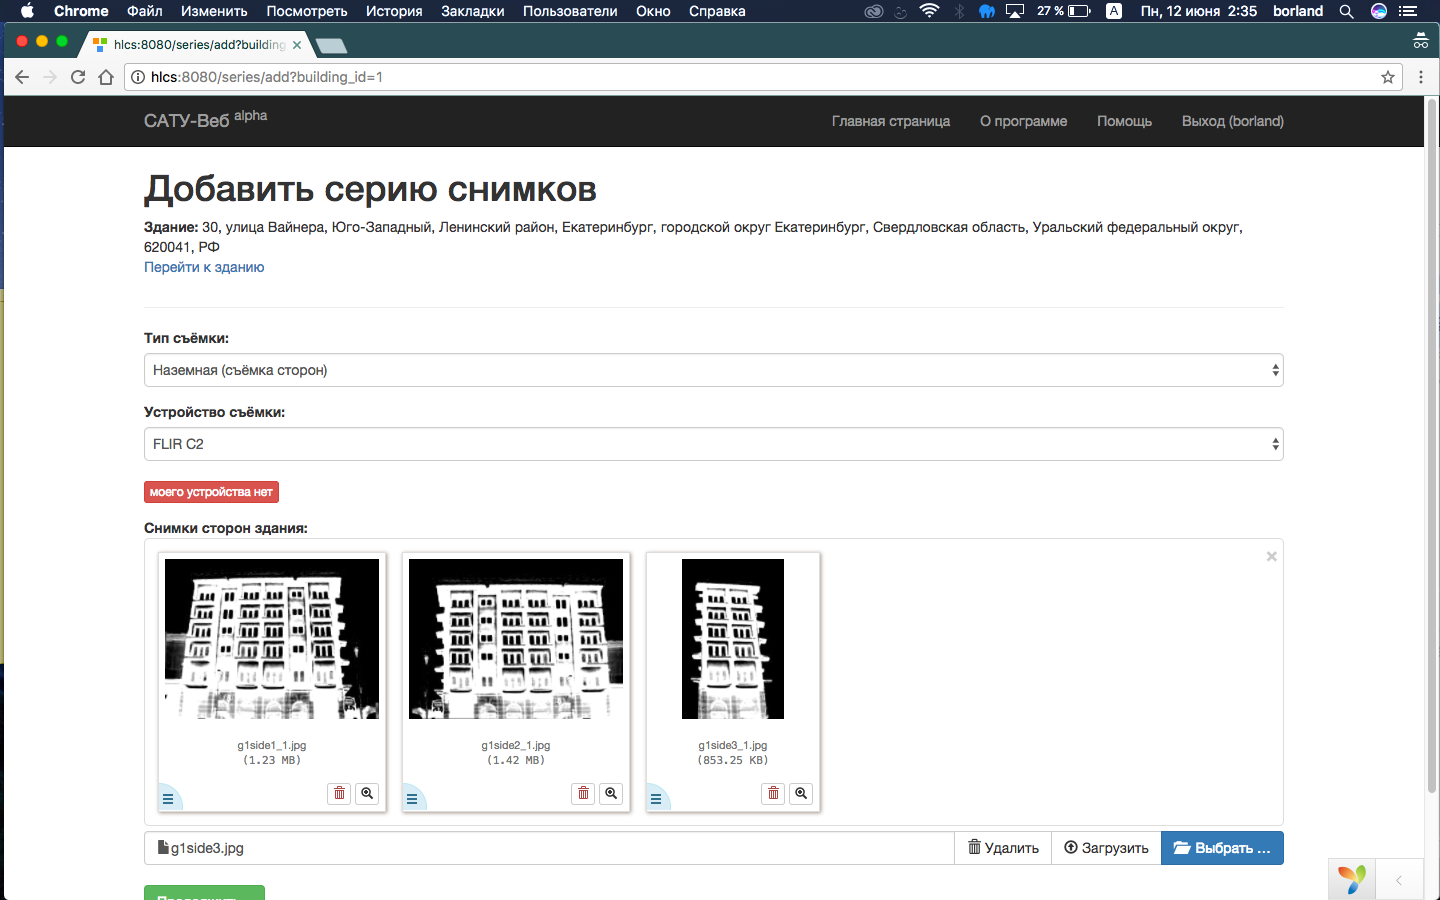
\includegraphics[width=1\textwidth]{images/scrshots/add-series_1}
		\caption{Форма добавления серии снимков (этап 1)}
		\label{scrshot:add-series_1}
	\end{figure}

	\begin{figure}[t!]
		\centering
		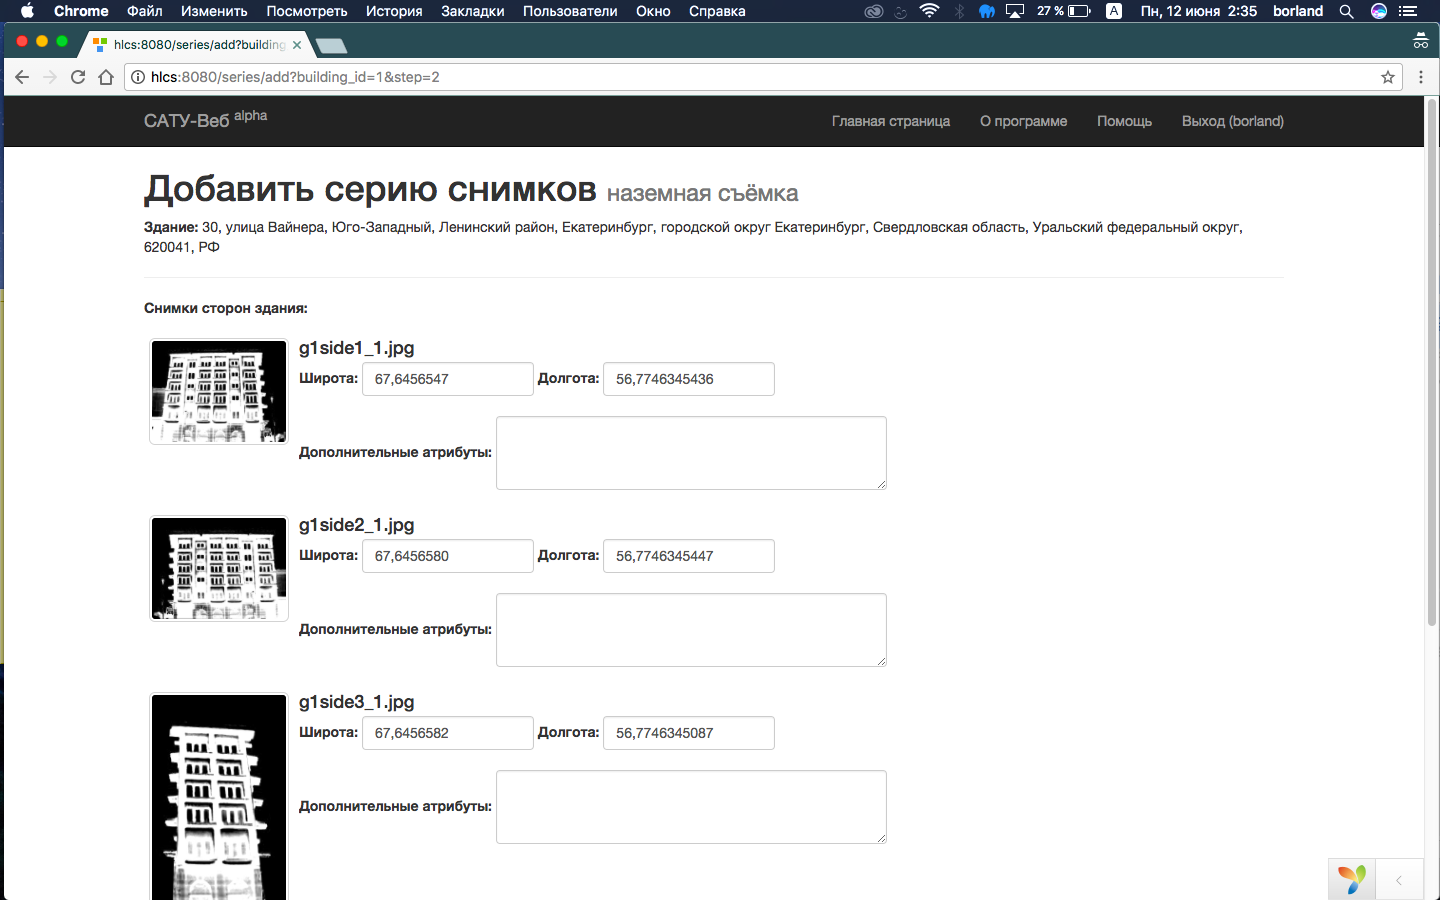
\includegraphics[width=1\textwidth]{images/scrshots/add-series_2}
		\caption{Форма добавления серии снимков (этап 2)}
		\label{scrshot:add-series_2}
	\end{figure}
 
	Форма загрузки изображений использует два способа выбора файлов: перетаскивание в область формы вручную; указание каталога, содержащего файл с помощью всплывающего при нажатии на кнопку “Выбрать” окна. После выбора в форме отображаются пиктограммы изображений и указывается их размер. При желании изображения можно удалить из формы.

	После успешного добавления здания в САТУ на главной странице в разделе “Недавно добавленные” отображаются последние зарегистрированные системой здания. При нажатии на кнопку с адресом здания карта мгновенно переносит обзор на него.
 
	Некоторые действия, такие как загрузка снимков и добавление зданий, недоступны пользователям, не представившимся в системе. Для этого предусмотрены страницы с формами регистрации и входа в систему (рисунки \ref{scrshot:register_1}, \ref{scrshot:login_1}).

	\begin{figure}[t!]
		\centering
		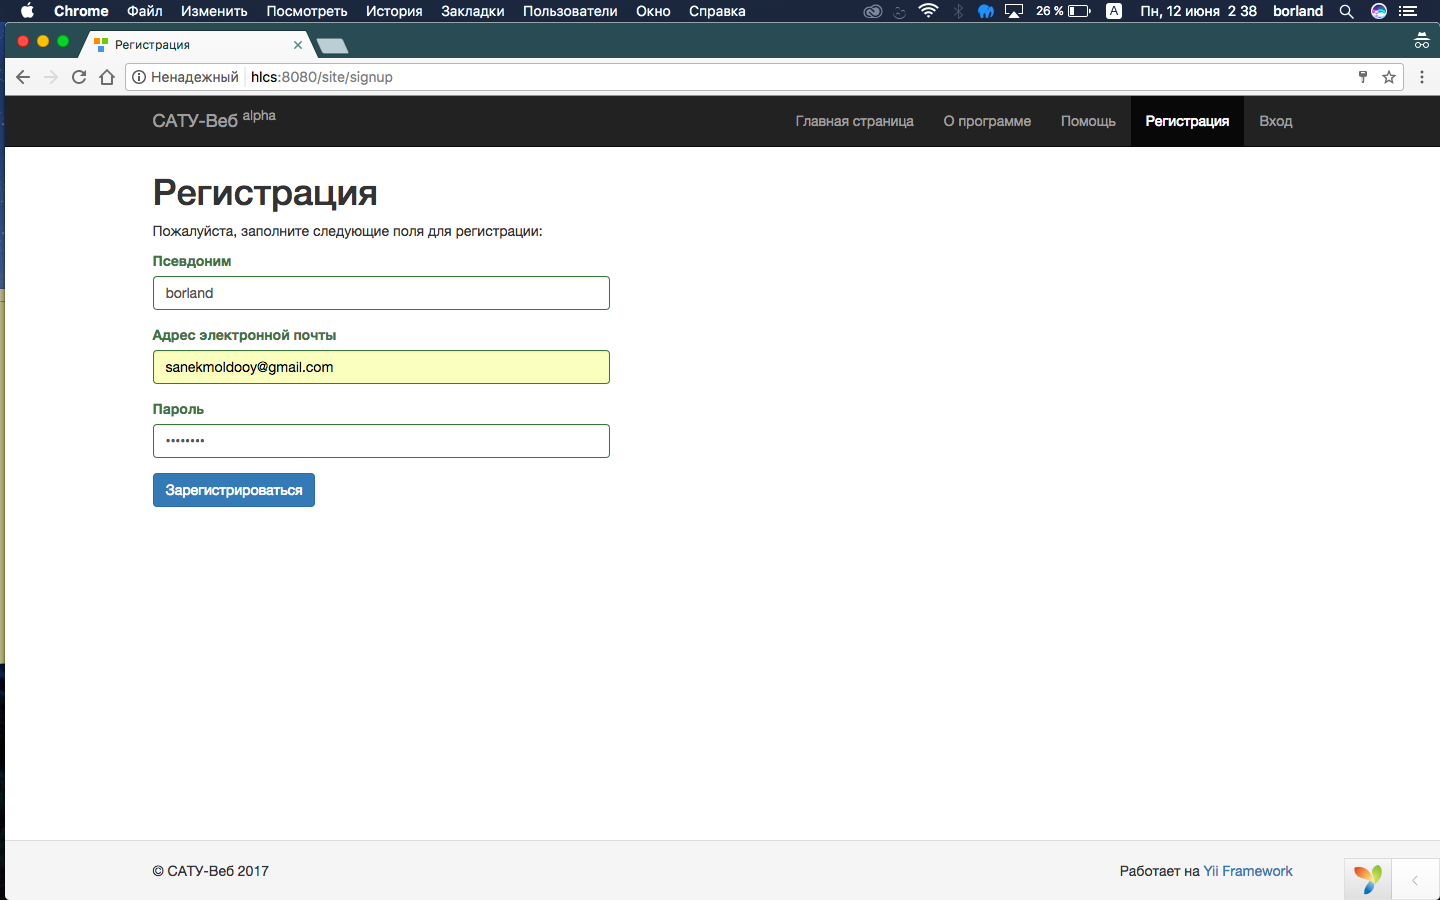
\includegraphics[width=1\textwidth]{images/scrshots/register_1}
		\caption{Форма добавления серии снимков (этап 1)}
		\label{scrshot:register_1}
	\end{figure}

	\begin{figure}[t!]
		\centering
		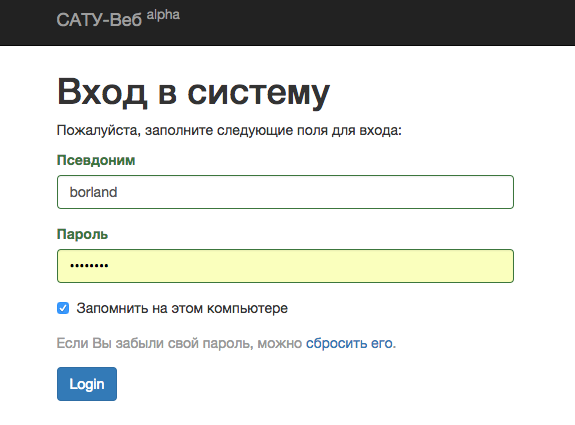
\includegraphics[width=1\textwidth]{images/scrshots/login_1}
		\caption{Форма добавления серии снимков (этап 2)}
		\label{scrshot:login_1}
	\end{figure}


\section{Результаты и выводы}



{
	\titleformat{\section}[block]{\centering\normalfont\large\bfseries}{\thesection}{10pt}{}
	\section*{\centering Заключение}
}
\addcontentsline{toc}{chapter}{Заключение}

\par
	На этапе исследования предметной области были изучены публикации, связанные с методами анализа утечек тепла. Был проведен обзор существующих систем анализа тепловых утечек, описаны критерии их оценки и выбран прототип разрабатываемой системы. Выявлены недостатки прототипа. Предложено решение, на основе которого сформулированы цели и задачи. На этапе моделирования созданы концептуальные, системно-структурные, функционально-структурные и алгоритмические модели прототипа и разрабатываемой системы. Полученный пакет моделей позволил перейти к этапу проектирования.
	На этапе проектирования были определены подсистемы разрабатываемой системы, описан их функционал и взаимосвязь. Определена программная платформа, средства и среда разработки. Создано Техническое задание на разработку системы. На стадии инженерной реализации были разработаны база данных, построена архитектура программного кода, реализованы экранные формы пользовательского интерфейса системы.

% Библиографический список
\renewcommand{\bibname}{Список использованных источников}
\titleformat{\chapter}[display]{\centering\normalfont\large\bfseries}{\chaptertitlename\ \thechapter}{}{}

\addcontentsline{toc}{chapter}{Список использованных источников}
%\bibliographystyle{bib/utf8gost705u}  %% стилевой файл для оформления по ГОСТу
%\bibliography{bib/biblio}     %% имя библиографической базы (bib-файла) 

\begin{thebibliography}{00}
	\bibitem{intro:thermo-analysis-federal}
	\emph{Анализ потребления тепловой энергии на отопление многоквартирных домов как способ повышения энергоэффективности в сфере ЖКХ} [Электронный ресурс] / Дирекция по проблемам ЖКХ //
	Аналитический центр при Правительстве Российской Федерации. --- 2013. --- Режим доступа:
	\url{http://gkh-altay.ru/d/205499/d/06_24_kr_stol_analitika_dor_abotannaya_po_rezultata_m.pdf} (дата обращения: 29.03.2017).

	\bibitem{intro:heating-drivers}
	\emph{Heating and cooling energy trends and drivers in buildings} / Ürge-Vorsatz D., Cabeza L. F., Serrano S., Barreneche C., Petrichenko K. //
	Renewable and Sustainable Energy Reviews --- Budapest, Hungary: Elsevier, 2015. --- \No{} 41 --- С. 85-98.

	\bibitem{intro:heat-loss-sources}
	\emph{What are the sources of home heat loss?} [Электронный ресурс] / Wilson L. //
	Shrink That Footprint --- Режим доступа: \url{http://shrinkthatfootprint.com/home-heat-loss} (дата обращения: 29.03.2017).

	\bibitem{intro:sources-residental}
	\emph{Detecting sources of heat loss in residential buildings from infrared imaging} [Электронный ресурс] / Chen S., Chen E. //
	Massachusetts Institute of Technology. Dept. of Mechanical Engineering --- 2011. --- Режим доступа: \url{http://hdl.handle.net/1721.1/68921} (дата обращения: 20.02.2017).

	\bibitem{intro:energy-use-perspective}
	\emph{Energy use in buildings in a long-term perspective} / Ürge-Vorsatz D., Petrichenko K., Staniec M., Eom J. //
	Current Opinion in Environmental Sustainability --- Budapest, Hungary: Elsevier, 2013. --- \No{} 5 --- С. 141-151.

	\bibitem{modeling:heat-technology}
	\emph{Geospatial Technologies to Improve Urban Energy Efficiency} / Hay G. J., Kyle C., Hemachandran B. et al. // Remote Sensing, 2011. --- \No{} 3(7) --- С. 1380-1405.

	\bibitem{problem:detection-windows-doors}
	\emph{Detection of windows and doors from thermal images by grouping geometrical features} / Sirmacek B., Hoegner L., Stilla U. //
	2011 Joint Urban Remote Sensing Event --- Germany, 2011.

	\bibitem{problem:aerial-oblique}
	\emph{Aerial oblique thermographic imagery for the generation of building 3D models to complement Geographic Information Systems} /  Lagüela S., Díaz-Vilariño L., Roca D., Armesto J. //
	QIRT Journal --- Germany, 2014.

	\bibitem{problem:thermal-leakages-facades}
	\emph{Thermal leakage detection on building facades using infrared textures generated by mobile mapping} / Hoegner L., Stilla U. //
	2009 Joint Urban Remote Sensing Event --- Germany, 2009.

	\bibitem{problem:knowledge-based-system}
	\emph{A knowledge-based system for the non-destructive diagnostics of façade isolation using the information fusion of visual and IR images} [Электронный ресурс] / Ribarić S., Marčetića D., Vedrinab D. S. // Faculty of Electrical Engineering and Computing, University of Zagreb --- 2008. --- Режим доступа: \url{http://www.sciencedirect.com/science/article/pii/S0957417408001425}, (дата обращения: 25.01.2017).

	\bibitem{problem:citizens-as-sensors}
	\emph{Citizens as sensors: the world of volunteered geography} / Goodchild, M. // GeoJournal, 2007. --- \No{} 69 --- C. 211–221.

	\bibitem{problem:vgi}
	\emph{VGI} [Электронный ресурс] : Материал из Википедии — свободной энциклопедии : Версия 755082720, сохранённая в 13:42 UTC 1 июня 2017 / Авторы Википедии // Википедия, свободная энциклопедия. — Электрон. дан. — Сан-Франциско: Фонд Викимедиа, 2017. — Режим доступа: \url{http://en.wikipedia.org/?oldid=755082720} (дата обращения: 02.06.2017).

	\bibitem{problem:myheat-utilities}
	\emph{MyHEAT - Utitlties} [Электронный ресурс] / MyHEAT, Inc. --- 2017 --- Режим доступа: \url{https://myheat.ca/utilities} (дата обращения: 02.05.2017).

	\bibitem{problem:nhm}
	\emph{National Heat Map} [Электронный ресурс] / Center for Sustainable Energy --- 2017 ---  Режим доступа: \url{https://www.cse.org.uk/projects/view/1183} (дата обращения: 02.05.2017).

	\bibitem{problem:heat}
	\emph{HEAT: A web based system for residental waste heat analysis using airborne thermal imagery} [Электронный ресурс] / Hemachandran B., Hay G. J., Kyle C. D. // Department of Geography, University of Calgary --- 2010. --- Режим доступа: \url{http://www.isprs.org/proceedings/XXXVIII/part1/01/01_04_Paper_178.pdf} (дата обращения: 05.05.2017).

	\bibitem{design:mvc}
	\emph{Model-View-Controller} [Электронный ресурс] : Материал из Википедии — свободной энциклопедии : Версия 85783223, сохранённая в 11:13 UTC 4 июня 2017 / Авторы Википедии // Википедия, свободная энциклопедия. — Электрон. дан. — Сан-Франциско: Фонд Викимедиа, 2017. — Режим доступа: \url{http://ru.wikipedia.org/?oldid=85783223} (дата обращения: 05.06.2017).

	\bibitem{design:rest}
	\emph{Architectural Styles and the Design of Network-based Software Architectures} / Fielding R. T. // The University of California, 2000.

	\bibitem{design:rest-uml}
	\emph{Overview of REST API Generation} [Электронный ресурс] / Visual Paradigm. Режим доступа: \url{https://www.visual-paradigm.com/support/documents/vpuserguide/276/3420/85153_overviewofre.html} (дата обращения: 05.06.2017).

	\bibitem{design:json}
	\emph{JSON} [Электронный ресурс] // Режим доступа: \url{http://json.org/} (дата
обращения: 27.03.2017).


\end{thebibliography}

\label{pagecount:expnote}

\pagebreak

\appendix

% Приложения
\input{inc/app-FSM}

\input{inc/app-TZ}

\end{document}
%%% Конец документа